% =====================================================================
%  REVIZE SURUM — 02.08.2026
%  Degisiklik kaydi: DEGISIKLIK_KAYDI.md
%  Tum sayilar tek bir dogrulanmis deney setinden gelir (results/*.json).
%  Onceki surumde farkli kosulardan gelen sayilar ayni tabloda karisiyordu.
% =====================================================================
\documentclass[journal]{IEEEtran}

\usepackage[utf8]{inputenc}
\usepackage[T1]{fontenc}
\usepackage{amsmath, amsfonts, amssymb}
\usepackage{booktabs}
\usepackage{cite}
\usepackage{graphicx}
\usepackage{bm}
\usepackage{hyperref}
\usepackage{array}
\usepackage{multirow}
\usepackage{placeins}
\usepackage{tabularx}
\usepackage{stfloats}
\usepackage[english]{babel}
\usepackage{microtype}
\emergencystretch=2em

\makeatletter
\renewcommand{\thetable}{\arabic{table}}
\renewcommand{\fnum@table}{Table \thetable.}
\long\def\@makecaption#1#2{%
\ifx\@captype\@IEEEtablestring%
\footnotesize\bgroup%
\setbox\@tempboxa\hbox{\normalfont\footnotesize {#1}\nobreakspace #2}%
\ifdim \wd\@tempboxa >\hsize%
\setbox\@tempboxa\hbox{\normalfont\footnotesize {#1}\nobreakspace}%
\parbox[t]{\hsize}{\normalfont\footnotesize\noindent\unhbox\@tempboxa#2}%
\else%
\hbox to\hsize{\normalfont\footnotesize\box\@tempboxa\hfil}%
\fi%
\par\addvspace{0.5\baselineskip}\egroup%
\@IEEEtablecaptionsepspace%
\else%
\@IEEEfigurecaptionsepspace%
\setbox\@tempboxa\hbox{\normalfont\footnotesize {#1.}\nobreakspace\nobreakspace #2}%
\ifdim \wd\@tempboxa >\hsize%
\setbox\@tempboxa\hbox{\normalfont\footnotesize {#1.}\nobreakspace\nobreakspace}%
\parbox[t]{\hsize}{\normalfont\footnotesize\noindent\unhbox\@tempboxa#2}%
\else%
\hbox to\hsize{\normalfont\footnotesize\box\@tempboxa\hfil}%
\fi%
\fi}
\makeatother

% =====================================================================
% ARTEFAKT ADRESLERI — TEK YERDE.
% Depo acilip Zenodo surumu yayinlandiktan sonra yalnizca bu iki satir
% duzenlenir. `makale/_verify_numbers.py` asagidaki varsayilan degerleri
% "yer tutucu" olarak yakalar ve doldurulana kadar dogrulama gecmez.
% =====================================================================
\newcommand{\repourl}{https://github.com/keremkartal/Anomaly-Detection}
% Surum DOI'si: v2.0.0 anlik goruntusune, yani bu makaledeki sayilari
% ureten kodun tam haline coozulur. Kavram DOI'si her zaman en son surume
% coozulur ve ikisi de veri erisim beyaninda verilir.
\newcommand{\zenododoi}{10.5281/zenodo.22637361}
\newcommand{\zenodoconcept}{10.5281/zenodo.22637360}

\begin{document}
\raggedbottom

% BASLIK NOTU: v1 basligi "A Controlled Multi-Seed Evaluation of Hybrid
% LSTM-GAT Architectures" idi. Calismanin merkezi bulgusu artik yalnizca
% cok-tohumlu degerlendirme degil; bolme secimi ve pencere kumelenmesinin
% sonuclari tersine cevirebildigi. Baslik buna gore guncellendi.
\title{How Much Does Fusion Design Matter? Partition, Seed, and Cluster Effects in the Evaluation of Hybrid LSTM--GAT Traffic Anomaly Detectors}

\author{
    Ayhan~Gültekin$^{1}$ $|$ Kerem~Kartal$^{2}$ $|$ Ahmet~Yusuf~Şimşek$^{3}$ $|$ Rümeysa~Yeşilova$^{3}$ $|$ Ahmet~Sayar$^{4}$ \\[2ex]
    \small
    $^{1}$Student Affairs Department, Kocaeli University, Kocaeli, Türkiye $|$
    $^{2}$Department of Software Engineering, Kocaeli University, Kocaeli, Türkiye $|$
    $^{3}$Department of Artificial Intelligence and Machine Learning, Kocaeli University, Kocaeli, Türkiye $|$
    $^{4}$Department of Artificial Intelligence Engineering, Bahçeşehir University, Istanbul, Türkiye \\[1.5ex]
    \textbf{Correspondence:} Ayhan Gültekin (ayhan.gultekin@kocaeli.edu.tr)
}

\maketitle

% =====================================================================
% ABSTRACT — YENIDEN YAZILDI
% Onceki surum "outperforming baselines" iddiasi tasiyordu; olculen
% sonuclar bu iddiayi desteklemedigi icin cerceve degistirildi.
% =====================================================================
\begin{abstract}
Hybrid spatio-temporal architectures for traffic anomaly detection are typically reported through a single training run on a single data partition, with overlapping sliding windows treated as independent observations. This paper asks how much of such evidence survives a controlled protocol. Using a physics-informed synthetic trajectory dataset over an OpenStreetMap-derived road network, we hold the task, optimization budget, checkpoint criterion, and threshold rule fixed; vary one component at a time across nine encoder configurations, four fusion operators, and two graph constructions; and report every result over multiple seeds. Because windows are cut with stride 10 from length-50 sequences and therefore overlap by $80\%$, all inference uses the \emph{trip} as the statistical unit, with cluster bootstrap, sign-flip permutation tests, and Holm correction. Four findings emerge. First, on the fixed partition---which contains 4{,}799 windows but only 14 trips---\emph{no} comparison remains significant once the correct unit and multiplicity correction are applied; seven comparisons that are significant at the window level are not. Second, under five-fold trip-grouped cross-validation, in which all 90 trips receive an out-of-fold prediction, the four fusion operators span $0.0205$ F1 with a within-configuration standard deviation of $0.04$--$0.05$, and none is distinguishable from any other: the sample-wise gate that motivated the original design ranks last on the fixed partition and first under cross-validation, so the choice of fusion operator is not resolvable on this data in either direction. Third, a reproducible degenerate failure mode of the gate is documented---it collapses to $\mathrm{F1}=0.0715$ at one seed, recurring at the same seed across an independent re-run---and localized: it occurs only when the gate locks onto a spatial branch with near-chance standalone discriminative power, and disappears on a graph construction where that branch is more informative. Fourth, no comparison survives at all. Under cross-validation the spatial branch shows no significant benefit on any anomaly subtype, and the one comparison nearest to significance runs against it. An earlier version of this study reported a spatial gain on abnormal-dwell detection; it was produced by applying a threshold averaged across folds rather than each fold's own, and disappears when that is corrected. We additionally report a zero-parameter threshold-rule reference ($\mathrm{F1}=0.8536$), gradient-boosting baselines that match the hybrid model to within $0.0014$ F1, probability calibration, and single-window latency. The study argues that architectural claims in this problem setting require multi-partition evidence at the correct statistical unit, and demonstrates on its own earlier results what happens when they do not have it.
\end{abstract}

\begin{IEEEkeywords}
  Traffic Anomaly Detection, Spatio-Temporal Modeling, Graph Attention Network (GAT), Long Short-Term Memory (LSTM), Multimodal Fusion, Ablation Study, Evaluation Methodology, Clustered Data, Cluster Bootstrap, Permutation Test, Reproducibility, Intelligent Transportation Systems.
\end{IEEEkeywords}

\section{Introduction}

Intelligent Transportation Systems (ITS) have become a fundamental component of modern urban mobility management by enabling large-scale monitoring and analysis of traffic conditions through heterogeneous data sources. These systems generate massive volumes of spatio-temporal traffic data, providing new opportunities for understanding driving behavior and enhancing road safety. Traffic anomalies---such as sudden stops or abnormal maneuvers---can disrupt traffic flow and create significant safety risks. Accurate and timely detection is therefore critical for decision-support mechanisms in ITS environments.

Recent studies have leveraged deep learning, particularly \textbf{Long Short-Term Memory (LSTM)} networks, to model sequential vehicle trajectories. However, road segments form complex graph-structured networks, making purely temporal reasoning insufficient for context-sensitive anomaly detection. To capture structural dependencies, \textbf{Graph Attention Networks (GAT)} and related graph-based approaches have been increasingly adopted alongside temporal encoders. As reflected in recent literature, current research increasingly moves toward both richer spatio-temporal anomaly modeling and more effective fusion strategies for integrating temporal behavior with spatial context \cite{huang_multivariate_2024, sun_framework_2025, nguyen_spatiotemporal_2026, liang_anomaly_2025}. Existing approaches frequently suffer from \textbf{``contextual blindness,''} where a model flags natural behavior as anomalous due to limited structural awareness, while many multimodal methods still rely on static or weakly adaptive fusion that cannot fully respond to changing traffic conditions \cite{sun_framework_2025, liang_anomaly_2025}.

% ---------------------------------------------------------------------
% YENI: makalenin cercevesi burada degisiyor.
% ---------------------------------------------------------------------
A recurring methodological pattern accompanies this progress. Architectural contributions in this area are commonly evaluated through a \emph{single} training run on a \emph{single} train/test partition, and improvements of one to three F1 points are reported as evidence that a proposed fusion or attention mechanism is responsible for the gain. Two properties of the anomaly-detection setting make such evidence fragile. First, anomaly prevalence is low, so the number of positive test instances is small and paired significance tests have limited power. Second, graph message passing on GPU is not bit-reproducible---scatter-based aggregation performs floating-point summation in a nondeterministic order---so repeated runs of an identical configuration do not return identical numbers. Under these conditions, a single-run difference cannot distinguish an architectural effect from seed and partition variance.

This paper therefore asks a narrower and more answerable question than ``is the proposed architecture better?'': \emph{which components of a hybrid LSTM--GAT anomaly detector actually carry the observed performance, and how much of the reported advantage survives a controlled protocol?} We keep the task formulation, dataset, grouped partition, optimizer, epoch budget, checkpoint criterion, and threshold-selection rule fixed, vary one component at a time, and report every result over multiple seeds with interval estimates and paired tests. The system under study is the hybrid design we previously proposed, denoted \textbf{STANet}, whose fusion stage is a sample-wise scalar modality gate; the evaluation, however, is deliberately symmetric and does not privilege that design.

The main contributions are:
\begin{itemize}
  \item \textbf{Controlled encoder benchmark.} Nine encoder configurations---covering the core operators of STGCN, DCRNN, and Graph WaveNet adapted to the present task---are compared under an identical protocol over five seeds. The comparison separates two questions that are usually reported together. The choice of \emph{spatial} operator is resolvable: graph attention exceeds Chebyshev convolution, diffusion convolution, and adaptive adjacency with significant margins. The choice of \emph{temporal} encoder is not: the LSTM, a GRU, and a Transformer encoder finish within $0.0015$ F1 of one another, an order of magnitude below the leader's own seed standard deviation.
  \item \textbf{Direct fusion ablation.} Four fusion operators---sample-wise gating, fixed concatenation, static weighted summation, and multi-head cross-attention---are compared with all other components frozen. Sample-wise gating ranks last, exhibits a degenerate collapse mode in one of five seeds, and its learned optimum coincides with a constant weight of $\approx 0.50$. Repeating the ablation on a second graph construction localizes the collapse: it occurs when the gate locks onto a spatial branch that carries almost no standalone signal, and disappears when that branch is made more informative.
  \item \textbf{Evidence on evaluation protocol.} We show that an ablation conclusion drawn from one fixed grouped partition is not reproduced under five-fold trip-grouped cross-validation covering all sequences. We further show that the windows used as observations overlap by $80\%$, so the window-level tests customary in this literature overstate the effective sample size; all inference here uses the trip as the unit, with cluster bootstrap, permutation tests, and Holm correction.
  \item \textbf{Reference points and transparency.} A zero-parameter threshold-rule classifier derived from the generation thresholds, gradient-boosting baselines on window aggregates, probability calibration, and single-window latency on GPU and CPU are reported alongside the learned models, together with a complete data card for the synthetic dataset. Every result file carries a protocol hash, and configurations appearing in several tables are trained once and shared, so the tables are consistent by construction rather than by assertion.
\end{itemize}

\section{Related Work}
The literature most relevant to this study covers both anomaly-detection models and the fusion strategies used to integrate temporal and spatial information.

\subsection{Temporal, Spatial, and Spatio-Temporal Anomaly Models}
Early traffic anomaly detection studies were predominantly driven by temporal modeling, where recurrent architectures such as LSTM-based networks were used to capture abrupt variations in velocity, acceleration, and short-term driving behavior. These models remain effective when anomalies are primarily reflected in kinematic changes, but they often overlook whether a maneuver is contextually plausible for the surrounding road environment. In parallel, graph-based and spatially aware methods improved structural understanding by modeling road connectivity, segment interactions, and topological constraints. Such approaches are better suited to representing where risky conditions may emerge, yet they can miss the sequential behavioral evolution that distinguishes a routine slowdown from a truly hazardous event.

Recent studies increasingly bridge these two views through spatio-temporal learning. Huang et al. \cite{huang_multivariate_2024} combine Dynamic GAT and Informer components to capture long-range temporal dependencies together with adaptive relational structure. Duan et al. \cite{sun_framework_2025} extend this direction through a multimodal deep-fusion framework with heterogeneous graph neural networks. Nguyen et al. \cite{nguyen_spatiotemporal_2026} further show that graph-based spatio-temporal integration can effectively represent coupled speed--volume patterns in urban traffic environments. Taken together, these studies confirm that anomaly detection benefits from combining behavioral evolution with structural context; how much weight each modality should receive, however, is usually settled by architectural configuration rather than measured directly.

\subsection{Fusion Strategies and Context Integration}
A second research direction focuses on how information from temporal and spatial branches should be fused. Liang et al. \cite{liang_anomaly_2025} adopt a lightweight spatio-temporal architecture that emphasizes compact feature fusion, whereas Cui et al. \cite{cui_lane-flow-learning_2026} use a spatial--temporal attention design for lane-aware trajectory prediction. These studies show that attention and feature-level coupling improve representation quality, yet the relative contribution of temporal and spatial cues is still largely determined by architectural configuration rather than by an explicit, empirically validated comparison against simpler fusion operators.

The mechanism examined in this paper is a \textbf{sample-wise scalar modality gate} applied after the LSTM and GAT outputs have been projected into a shared 64-dimensional space. It produces one scalar per sample and broadcasts that value across all latent features; it is not a feature-level attention vector, a time-step attention mechanism, or a graph-neighborhood coefficient. Table \ref{tab:comparison} places this mechanism among related designs. A central empirical question of this study is whether that modality-level distinction translates into a measurable advantage; Section~\ref{sec:fusion_ablation} reports that, under a controlled protocol, it does not.

% Domain adaptation baglaminda eklendi (Hakem 2, Madde 2) — sim-to-real
% aktarim tartismasi Bolum VIII-C'de.
Beyond fusion design, transfer between simulated and real operating conditions is an open problem for simulation-trained detectors. Digital twin-assisted graph contrastive domain adaptation has shown promise for adapting simulation-derived representations to small-sample target domains in adjacent diagnostic fields \cite{gcda_bearing}, and we return to this direction in Section~\ref{sec:future_directions}.

\begin{table*}[!t]
\centering
\caption{Summary of related spatio-temporal anomaly detection methods}
\label{tab:comparison}
\renewcommand{\arraystretch}{1.25}
\footnotesize
\setlength{\tabcolsep}{3pt}
\begin{tabularx}{0.97\textwidth}{@{}>{\raggedright\arraybackslash}p{0.15\textwidth}>{\centering\arraybackslash}p{0.06\textwidth}>{\raggedright\arraybackslash}X>{\raggedright\arraybackslash}X>{\raggedright\arraybackslash}X>{\raggedright\arraybackslash}X@{}}
  \toprule
  \textbf{Study} & \textbf{Year} & \textbf{Core Arch.} & \textbf{Temporal} & \textbf{Spatial} & \textbf{Fusion} \\ \midrule
  Huang et al.~\cite{huang_multivariate_2024} & 2024 & Dynamic GAT--Informer & Informer & Dynamic GAT & Integrated gated feature fusion with graph-neighborhood attention \\
  Duan et al.~\cite{sun_framework_2025} & 2025 & Multimodal deep fusion + HGNN & Traffic flow / speed dynamics & Heterogeneous GNN & Integrated multimodal feature fusion \\
  Nguyen et al.~\cite{nguyen_spatiotemporal_2026} & 2026 & Spatiotemporal prediction model & Time-series analysis & Graph-based dependency modeling & Integrated spatio-temporal feature fusion \\
  Liang et al.~\cite{liang_anomaly_2025} & 2025 & Lightweight ST network & TCN / CNN & Spatio-temporal features & Compact feature-level fusion \\
  Cui et al.~\cite{cui_lane-flow-learning_2026} & 2026 & Lane-flow fusion attention & Temporal self-attention & Lane-level spatial attention & Feature-level attention fusion \\
  \textbf{This study} & \textbf{2026} & \textbf{Hybrid LSTM--GAT, evaluated component-wise} & \textbf{Stacked LSTM (vs.\ GRU, gated TCN, dilated conv, Transformer)} & \textbf{GAT (vs.\ Chebyshev, diffusion, adaptive adjacency, none)} & \textbf{Four operators compared directly: gated, concat, weighted sum, cross-attention} \\ \bottomrule
\end{tabularx}
\end{table*}

\FloatBarrier

% =====================================================================
% BOLUM III — DEGISMEDI (matematik ve notasyon aynen korundu)
% =====================================================================
\section{Problem Formulation}

Urban traffic systems can be modeled as complex spatio-temporal processes in which vehicle movements evolve while simultaneously occurring within the structural constraints of a road network \cite{zhang_automatic_2022, zhang_traffic_2025}. In this study, the traffic anomaly detection problem is formulated as a context-aware learning task that jointly models vehicle trajectory dynamics and road network topology \cite{ren_graph_2024}. The mathematical notations used throughout this formulation are summarized in Table \ref{tab:notations}.

\begin{table}[!htbp]
  \centering
  \caption{Summary of mathematical notation}
  \label{tab:notations}
  \renewcommand{\arraystretch}{1.2}
  \begin{tabular}{@{}p{0.36\columnwidth}p{0.58\columnwidth}@{}}
    \toprule
    \textbf{Symbol} & \textbf{Description} \\ \midrule
    $\mathcal{G} = (\mathcal{V}, \mathcal{E})$ & Directed graph representing the road network \\
    $\mathcal{V}, \mathcal{E}$ & Set of nodes (road segments) and edges (connectivity) \\
    $N, \mathbf{A}$ & Number of nodes and adjacency matrix encoding connectivity \\
    $\mathbf{s}_i, \mathcal{S}$ & Structural feature vector of node $i$ and the set of all structural features \\
    $\mathcal{T} = \{\mathbf{x}_1, \dots, \mathbf{x}_\tau\}$ & Vehicle trajectory sequence of length $\tau$ \\
    $\mathbf{x}_t, \mathbf{X} \in \mathbb{R}^{\tau \times 4}$ & Per-step kinematic vector and stacked temporal feature matrix \\
    $v_t, a_t, \theta_t, id_t$ & Velocity, acceleration, heading angle, and road-segment ID at time $t$ \\
    $x_{sin}, x_{cos}$ & Trigonometric heading components used for continuous angular representation \\
    \shortstack[l]{$type_i, length_i$\\$deg_i, context_i$} & \shortstack[l]{Road category and segment length;\\node degree and contextual attributes} \\
    $\mathbf{h}_t, \mathbf{h}_{temp}, \mathbf{h}_{spat}$ & LSTM hidden state, temporal embedding, and spatial embedding \\
    $\Theta_{temp}, \Theta_{spat}$ & Learnable parameter sets of the LSTM and GAT branches \\
    $\alpha_{ij}, \mathcal{N}_i$ & Graph-attention coefficient from node $j$ to node $i$ and neighborhood of node $i$ \\
    $\mathbf{W}, \vec{a}, \mathbf{h}_i'$ & GAT transform matrix, attention vector, and updated node representation \\
    $d$ & Shared latent dimension used before multimodal fusion \\
    $\mathbf{h}'_{temp}, \mathbf{h}'_{spat}$ & Projected temporal and spatial embeddings in shared latent space \\
    \shortstack[l]{$\mathbf{W}_t, \mathbf{b}_t$\\$\mathbf{W}_s, \mathbf{b}_s$} & Learnable projection parameters for temporal/spatial branches \\
    $g_{gate}, \mathbf{W}_g, b_g$ & Sample-wise scalar modality weight and gating-network parameters \\
    $\mathbf{z}$ & Joint spatio-temporal fused embedding \\
    \shortstack[l]{$f_{LSTM}(\cdot), f_{GAT}(\cdot)$\\$f_{fusion}(\cdot), g(\cdot)$} & \shortstack[l]{Temporal encoder, spatial encoder,\\fusion, and classification mappings} \\
    $\sigma(\cdot)$ & Activation function (sigmoid where specified) \\
    \shortstack[l]{$y, \hat{y}$\\$y_i, \hat{y}_i$} & Ground-truth and predicted labels (global and sample-level forms) \\
    $\mathcal{L}, M$ & Loss function and mini-batch size \\
    $w_{pos}$ & Positive-class weight in the WBCE loss \\
    $\Phi$ & Overall mapping function for anomaly detection \\ \bottomrule
  \end{tabular}
\end{table}

\subsection{Road Network Representation}
The road network is represented as a directed graph $\mathcal{G} = (\mathcal{V}, \mathcal{E})$, where $\mathcal{V}$ is a set of $N$ nodes (road segments) and $\mathcal{E}$ denotes the set of edges representing physical connectivity \cite{li_graph_2023, park_graph_2025}. Each node $v_i \in \mathcal{V}$ is associated with a structural feature vector $\mathbf{s}_i$:
\begin{equation}
  \mathbf{s}_i = [type_i, length_i, deg_i, context_i]
\end{equation}
where $type_i$ denotes the road category, $length_i$ is the segment length, $deg_i$ is the node degree, and $context_i$ represents additional intersection characteristics \cite{chen_enhancing_2026, zhong_multi-factor_2025}. Spatial dependencies are encoded via an adjacency matrix $\mathbf{A}$ \cite{pan_dc-stgcn_2021, chang_stfdsgcn_2025}.

\subsection{Vehicle Trajectory Modeling}
Vehicle movement is represented as a trajectory sequence $\mathcal{T} = \{\mathbf{x}_1, \mathbf{x}_2, \dots, \mathbf{x}_\tau\}$, where $\tau$ is the sequence length and each observation $\mathbf{x}_t$ describes the kinematic state at time $t$ \cite{zhou_hybrid_2022, taheri_sarteshnizi_applicability_2026}:
\begin{equation}
  \mathbf{x}_t = [v_t, a_t, \theta_t, id_t]
\end{equation}
where $v_t$ is speed, $a_t$ is acceleration, $\theta_t$ is the heading angle, and $id_t$ is the identifier of the road segment where the vehicle is located.

\subsection{Spatio-Temporal Feature Representation}
Anomaly detection requires the integration of behavioral dynamics and structural context \cite{hu_dynamic_2026, zhu_spatio-temporal_2026}. We define the learning task as finding a joint embedding $\mathbf{z}$:
\begin{equation}
  \mathbf{z} = f(\mathbf{h}_{temp}, \mathbf{h}_{spat})
\end{equation}
where $\mathbf{h}_{temp} = \text{LSTM}(\mathcal{T})$ and $\mathbf{h}_{spat} = \text{GAT}(\mathcal{G}, \mathbf{A})$ \cite{xia_attention-based_2023, wang_multi-scale_2025}. The function $f(\cdot)$ denotes the fusion operator, which is treated in this study as an \emph{experimental variable} rather than a fixed design choice.

\subsection{Traffic Anomaly Detection Objective}
The detection task is formulated as a binary classification:
\begin{equation}
  \hat{y} = \sigma(g(\mathbf{z}))
\end{equation}
where $g(\cdot)$ is the classification head and $\hat{y} \in [0, 1]$. At the task-formulation level:
\begin{equation}
  \label{eq:generic_bce}
  \mathcal{L} = -\frac{1}{M} \sum_{i=1}^{M} [y_i \log(\hat{y}_i) + (1 - y_i) \log(1 - \hat{y}_i)]
\end{equation}
where $y_i \in \{0, 1\}$ is the ground truth label and $M$ is the number of samples \cite{feng_traffic_2024, sun_framework_2025, ma_utfp-ad_2025}. Equation~\ref{eq:generic_bce} is the generic task-level formulation only; because the training partition is imbalanced, the implemented objective is the weighted binary cross-entropy in Eq.~\ref{eq:wbce}.

\subsection{Problem Definition}
Given a road network $\mathcal{G}$, vehicle trajectory $\mathcal{T}$, and road features $\mathcal{S}$, the objective is to learn a mapping $\Phi: \{\mathcal{T}, \mathcal{G}, \mathcal{S}\} \rightarrow \{0, 1\}$ \cite{guo_crfpi-net_2026, ren_graph_2024}.

% =====================================================================
% BOLUM IV — MIMARI ANLATIMI KORUNDU
% Yalnizca kapinin "ne basardigi" iddialari kaldirildi; mekanizma
% tarifi aynen duruyor cunku dogru.
% =====================================================================
\section{Architecture Under Study}

This section describes the hybrid architecture whose components are evaluated in Section~\ref{sec:results}. The model jointly encodes temporal vehicle dynamics and spatial road-network topology through parallel branches and combines them with a configurable fusion operator. We describe the mechanism here and defer all claims about its effectiveness to the experimental sections; the protocol governing those experiments is given in Section~\ref{sec:protocol}.

\subsection{Overall Architecture}
As illustrated in Fig. \ref{fig:stanet_framework}, the framework consists of (i) a temporal module for sequence modeling, (ii) a spatial module for structural graph learning, and (iii) a fusion module that combines the two projected representations.

\begin{figure*}[t]
  \centering
  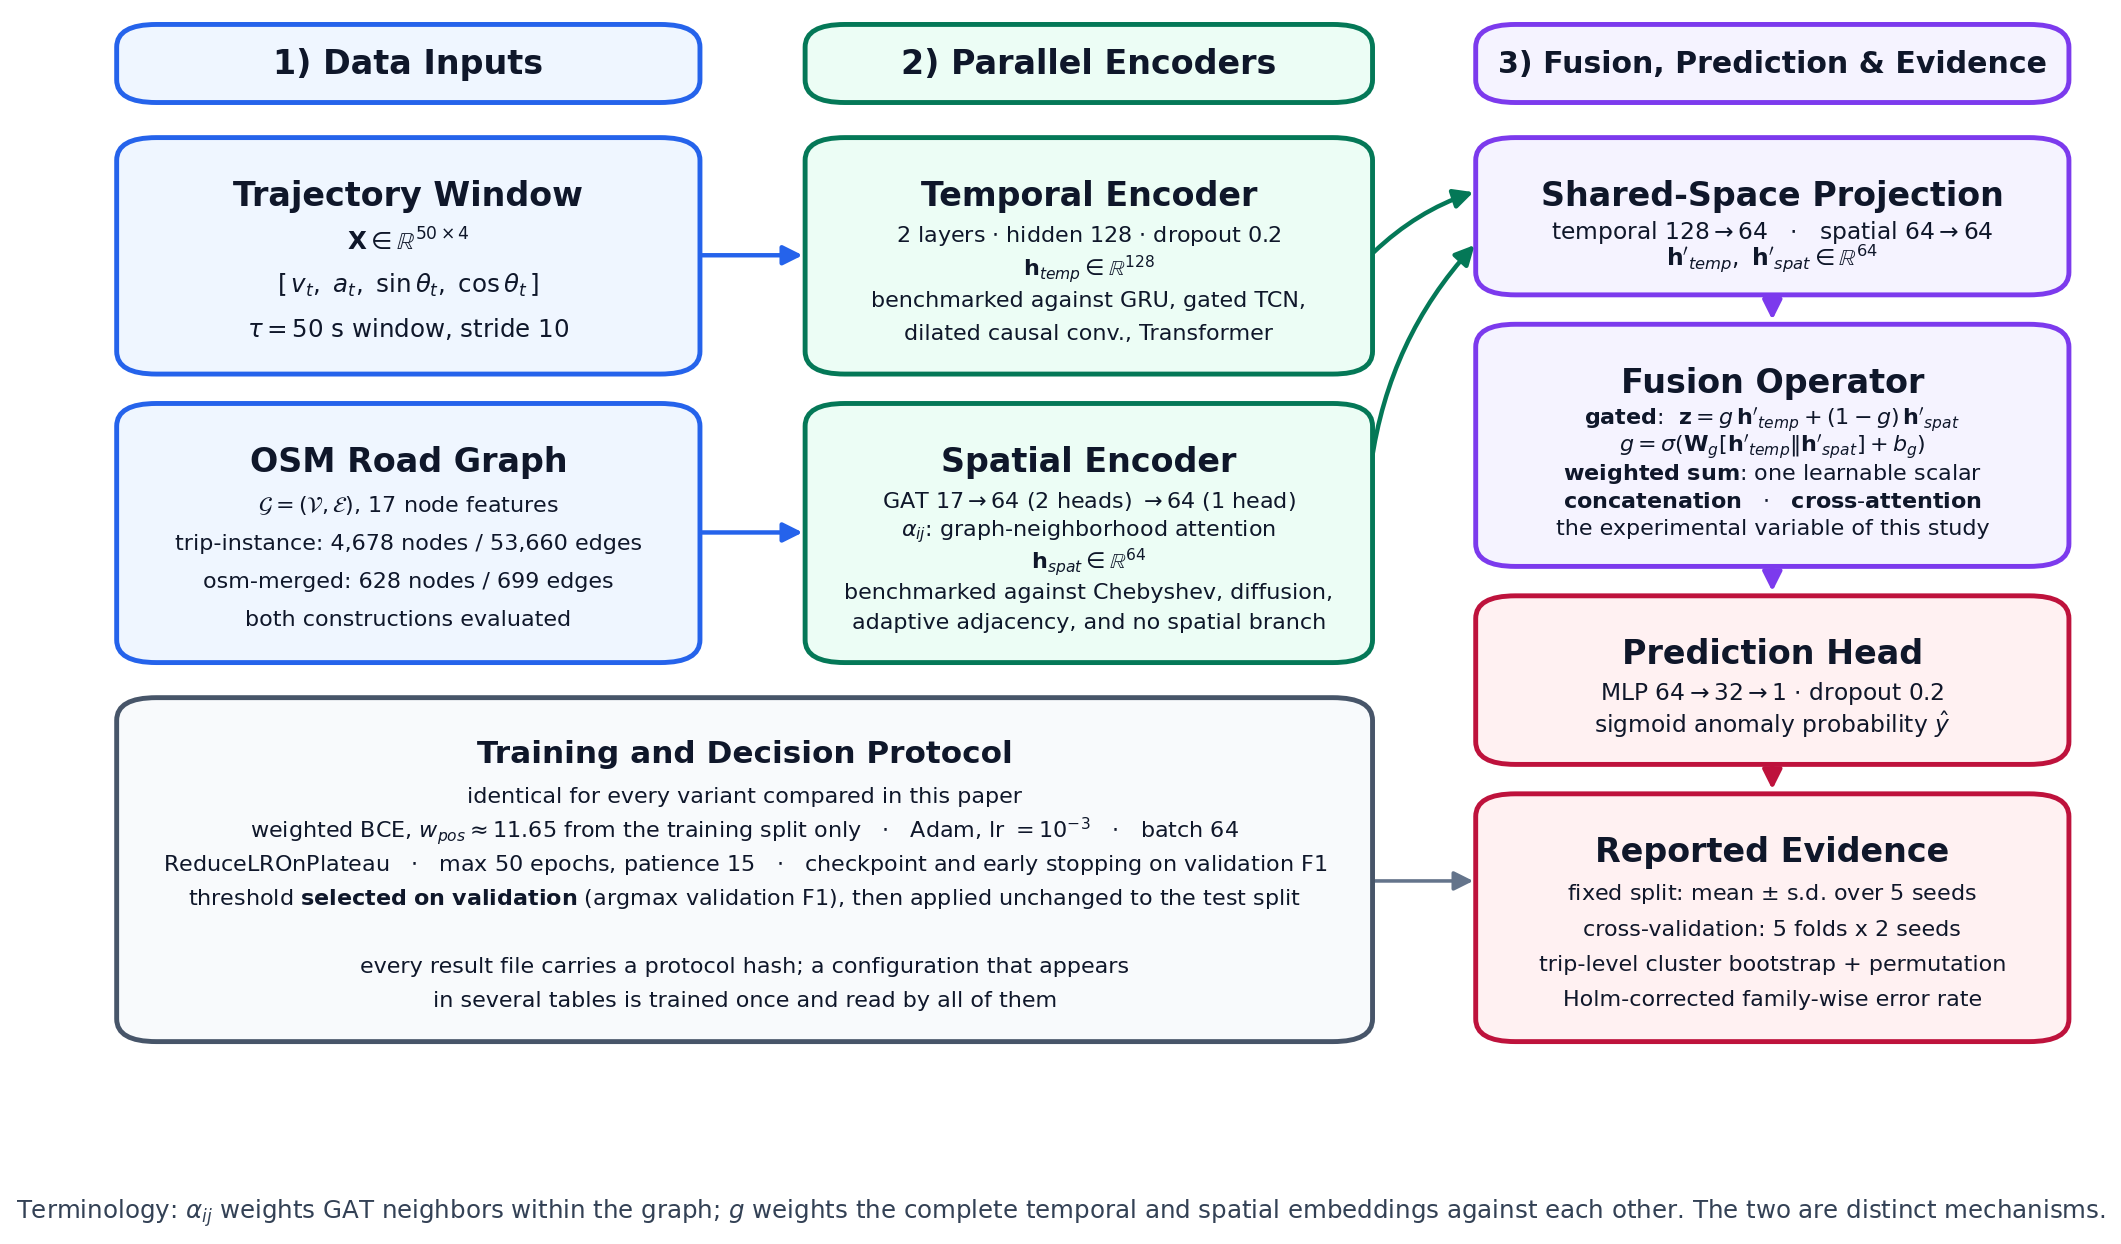
\includegraphics[width=0.98\textwidth]{stanet_framework_q1.png}
  \caption{Overall architecture. The GAT neighborhood coefficients $\alpha_{ij}$ are distinct from the sample-wise scalar modality gate $g_{gate}$; the fusion block is the experimental variable of Section~\ref{sec:fusion_ablation}.}
  \label{fig:stanet_framework}
\end{figure*}

Given a vehicle trajectory sequence $\mathcal{T}$ and the road network graph $\mathcal{G}$, the model learns two complementary latent embeddings:
\begin{align}
  \mathbf{h}_{temp} &= f_{LSTM}(\mathcal{T}; \Theta_{temp}) \\
  \mathbf{h}_{spat} &= f_{GAT}(\mathcal{G}, \mathbf{A}; \Theta_{spat})
\end{align}
where $\Theta_{temp}$ and $\Theta_{spat}$ denote the learnable parameter sets of the two branches \cite{wang_multi-scale_2025, he_c_2025}. These embeddings are integrated through the fusion operator:
\begin{equation}
  \mathbf{z} = f_{fusion}(\mathbf{h}_{temp}, \mathbf{h}_{spat})
\end{equation}
The fused representation $\mathbf{z}$ is then mapped by a classification head to the anomaly probability $\hat{y}$.

\subsection{Temporal Module}

\subsubsection{Kinematic Feature Representation}
The temporal branch processes four kinematic features at each time step $t$:
\begin{equation}
  \mathbf{x}_t = [v_t, a_t, \sin(\theta_t), \cos(\theta_t)]
\end{equation}
Representing the heading angle $\theta_t$ using its trigonometric components prevents periodic discontinuities at the angular boundaries \cite{taheri_sarteshnizi_applicability_2026}. Each driving window is represented as $\mathbf{X} \in \mathbb{R}^{\tau \times 4}$ with $\tau = 50$.

\subsubsection{LSTM-Based Sequence Encoding}
A two-layer stacked LSTM encoder is used \cite{zhou_hybrid_2022, taheri_sarteshnizi_applicability_2026, hirata_traffic_2025}:
\begin{equation}
  \mathbf{h}_t = \text{LSTM}(\mathbf{x}_t, \mathbf{h}_{t-1})
\end{equation}
Each layer contains 128 hidden units with dropout $0.2$ between recurrent layers. The final hidden state of the second layer is exported as the temporal embedding, $\mathbf{h}_{temp} = \mathbf{h}_\tau$. Table \ref{tab:lstm_config} summarizes the branch. Section~\ref{sec:encoder_benchmark} replaces this encoder with four alternatives while keeping everything else fixed.

\begin{table}[!htbp]
  \centering
  \caption{Summary of LSTM branch configuration}
  \label{tab:lstm_config}
  \renewcommand{\arraystretch}{1.15}
  \resizebox{\columnwidth}{!}{%
  \begin{tabular}{@{}lll@{}}
    \toprule
    \textbf{Component} & \textbf{Setting} & \textbf{Role / Output} \\ \midrule
    Input window & $\tau = 50$, 4 features & Tensor shape $[B, 50, 4]$ \\
    Input features & $v_t$, $a_t$, $x_{sin}$, $x_{cos}$ & Driving-profile representation \\
    Stacked LSTM & input size $=4$, hidden size $=128$ & Temporal dependency learning \\
    Number of layers & 2 & Hierarchical sequence encoding \\
    Dropout & $p = 0.2$ & Regularization between LSTM layers \\
    Temporal embedding & $\mathbf{h}_{temp} \in \mathbb{R}^{128}$ & Output tensor $[B, 128]$ \\
    Parameters & 200{,}704 & 89.2\% of the full model \\
    \bottomrule
  \end{tabular}}
\end{table}

\subsection{Spatial Module}

\subsubsection{Graph-Based Contextual Features}
The spatial module uses a GAT to encode the road network structure \cite{zhang_automatic_2022, li_graph_2023, zhong_multi-factor_2025}. Each node $v_i$ is associated with a 17-dimensional structural vector $\mathbf{s}_i$ capturing road-type descriptors, topological metrics (betweenness and closeness centrality), and contextual constraints (traffic-light indicators, tunnel information, rarity scores).

\subsubsection{Graph Attention Mechanism}
The GAT layers compute adaptive attention coefficients $\alpha_{ij}$ over adjacent road segments \cite{xia_attention-based_2023, ren_graph_2024, chen_gms_2026}:
\begin{equation}
  \alpha_{ij} = \frac{\exp\left(\text{LeakyReLU}\left(\vec{a}^T [\mathbf{W}\mathbf{s}_i \Vert \mathbf{W}\mathbf{s}_j]\right)\right)}{\sum_{k \in \mathcal{N}_i} \exp\left(\text{LeakyReLU}\left(\vec{a}^T [\mathbf{W}\mathbf{s}_i \Vert \mathbf{W}\mathbf{s}_k]\right)\right)}
\end{equation}
\begin{equation}
  \mathbf{h}_i' = \sigma \left( \sum_{j \in \mathcal{N}_i} \alpha_{ij} \mathbf{W}\mathbf{s}_j \right)
\end{equation}
Two consecutive GAT layers are used: the first maps the 17-dimensional node attributes to a 64-dimensional intermediate representation (32 hidden channels, 2 attention heads); the second produces the final 64-dimensional spatial embedding. The embedding of the road segment occupied by the vehicle is extracted as $\mathbf{h}_{spat}$. Table \ref{tab:gnn_config} summarizes the branch.

\begin{table}[!htbp]
  \centering
  \caption{Summary of GAT branch configuration}
  \label{tab:gnn_config}
  \renewcommand{\arraystretch}{1.15}
  \resizebox{\columnwidth}{!}{%
  \begin{tabular}{@{}lll@{}}
    \toprule
    \textbf{Component} & \textbf{Setting} & \textbf{Role / Output} \\ \midrule
    Graph input & $4{,}678$ nodes, $53{,}660$ edges & Trip-specific segment instances \\
    Distinct physical roads & 628 unique \texttt{osm\_segment\_id} & See Section~\ref{sec:graph_construction} \\
    Node features & 17 dimensions & Structural and contextual descriptors \\
    GAT layer 1 & GATConv$(17, 32,$ heads$=2)$ & Intermediate tensor $[N, 64]$ \\
    GAT layer 2 & GATConv$(64, 64,$ heads$=1)$ & Spatial embedding tensor $[N, 64]$ \\
    Spatial embedding & $\mathbf{h}_{spat} \in \mathbb{R}^{64}$ & Output of active road segment \\
    Parameters & 5{,}568 & 2.5\% of the full model \\
    \bottomrule
  \end{tabular}}
\end{table}

\subsection{Fusion Module}
\label{sec:fusion_module}
Since $\mathbf{h}_{temp}$ and $\mathbf{h}_{spat}$ originate from different branches, they are first projected into a common latent dimensionality $d = 64$:
\begin{align}
  \mathbf{h}'_{temp} &= \text{ReLU}(\mathbf{W}_t \mathbf{h}_{temp} + \mathbf{b}_t) \\
  \mathbf{h}'_{spat} &= \text{ReLU}(\mathbf{W}_s \mathbf{h}_{spat} + \mathbf{b}_s)
\end{align}

Four fusion operators are considered. The \textbf{sample-wise scalar modality gate} originally proposed computes Eq.~\ref{eq:gate} and applies it in Eq.~\ref{eq:gated_fusion}. The gate is a two-layer network, not the single projection written in the previous version of this paper: $\mathbf{W}_1 \in \mathbb{R}^{32 \times 128}$ and $\mathbf{w}_2 \in \mathbb{R}^{32}$, giving the $4{,}161$ parameters listed in Table~\ref{tab:fusion_config}. A reviewer noted the discrepancy between the equation and the table; the table and the released code were correct.
\begin{equation}
  \label{eq:gate}
  g_{gate} = \sigma\!\left(\mathbf{w}_2^{\top}\,\tanh\!\left(\mathbf{W}_1 [\mathbf{h}'_{temp} \Vert \mathbf{h}'_{spat}] + \mathbf{b}_1\right) + b_2\right)
\end{equation}
\begin{equation}
  \label{eq:gated_fusion}
  \mathbf{z} = g_{gate} \cdot \mathbf{h}'_{temp} + (1 - g_{gate}) \cdot \mathbf{h}'_{spat}
\end{equation}
where $g_{gate}\in[0,1]$ has tensor shape $[B,1]$: exactly one scalar per sample, broadcast across all 64 dimensions. The three comparison operators are \textbf{fixed concatenation} ($\mathbf{z} = [\mathbf{h}'_{temp} \Vert \mathbf{h}'_{spat}]$, no reweighting), \textbf{static weighted summation} ($\mathbf{z} = s\,\mathbf{h}'_{temp} + (1-s)\,\mathbf{h}'_{spat}$ with a single global learnable scalar $s$), and \textbf{multi-head cross-attention} (four heads, temporal embedding as query, both embeddings as key/value).

We note a structural relation that motivates the ablation. If $g_{gate}$ converges to a constant $\bar{g}$, then Eq.~\ref{eq:gated_fusion} followed by a linear classifier $\mathbf{W}$ yields $\mathbf{W}\mathbf{z} = \bar{g}\,\mathbf{W}\mathbf{h}'_{temp} + (1-\bar{g})\,\mathbf{W}\mathbf{h}'_{spat}$, which fixed concatenation can reproduce exactly by setting its two weight blocks to $\bar{g}\mathbf{W}$ and $(1-\bar{g})\mathbf{W}$. Concatenation therefore spans a strictly larger function class than constant-gate fusion, and any advantage of gating must come from genuinely sample-dependent behavior. Section~\ref{sec:gate_behaviour} tests whether such behavior is observed.

The fused representation passes through a two-layer MLP ($64 \rightarrow 32 \rightarrow 1$, ReLU, dropout $0.2$) to produce the anomaly probability. Table \ref{tab:fusion_config} summarizes the stage.

\begin{table}[!htbp]
  \centering
  \caption{Summary of the fusion stage and the four operators compared}
  \label{tab:fusion_config}
  \renewcommand{\arraystretch}{1.15}
  \resizebox{\columnwidth}{!}{%
  \begin{tabular}{@{}lll@{}}
    \toprule
    \textbf{Component} & \textbf{Setting} & \textbf{Fusion parameters} \\ \midrule
    Temporal projection & Linear $128 \rightarrow 64$ + ReLU & --- \\
    Spatial projection & Linear $64 \rightarrow 64$ + ReLU & --- \\
    Gated (proposed) & Linear $128\rightarrow32$ + tanh, $32\rightarrow1$ + sigmoid & 4{,}161 \\
    Fixed concatenation & $[\mathbf{h}'_{temp} \Vert \mathbf{h}'_{spat}]$ & 0 \\
    Static weighted sum & single learnable scalar $s$ & 1 \\
    Cross-attention & 4-head, $d=64$ & 16{,}640 \\
    Classifier & MLP $64/128 \rightarrow 32 \rightarrow 1$ & --- \\
    \bottomrule
  \end{tabular}}
\end{table}

% =====================================================================
% BOLUM V — VERI. Buyuk olcude korundu; veri karti icerigi eklendi,
% graf yapisi ve kural baseline sayilari duzeltildi.
% =====================================================================
\section{Dataset and Preprocessing}

\subsection{Data Sources}
The empirical evaluation relies on a \textbf{physics-informed synthetic vehicle trajectory dataset} and \textbf{OpenStreetMap (OSM)} road network topology.

\subsubsection{Vehicle Trajectory Dataset}
\nocite{wen_hdsvt_2025,feng_traffic_2024_dup2,yu_spatio-temporal_2018,li_diffusion_2018,wu_graph_2019,francies_framework_2025,pipes_car_following_1967,aashto_green_book_2018}
\textbf{No pre-existing real-world source dataset was used.} To obtain trajectory data with fully known ground-truth anomaly labels---difficult to obtain at scale from real sensor logs because of privacy constraints, sparse anomaly incidence, and the absence of verified incident annotations---this study employs a physics-informed synthetic trajectory-generation framework. Vehicle motion is simulated over the OSM-derived Kocaeli road network using a Markov-chain behavioral model in which each vehicle transitions between four kinematic states (constant speed, acceleration, deceleration, stop) at one-second resolution. State-transition probabilities are conditioned on the local traffic regime (free-flow, transition, congested), defined through a log-normal traffic-intensity distribution and a speed--density relationship adapted from Pipes' car-following model \cite{pipes_car_following_1967}:
\begin{equation}
  \bar{v}_s = (v_{\max} - 0.08v_{\max})\left(1-\frac{\tau}{10}\right)^4,
\end{equation}
where $v_{\max}$ is the segment's speed limit and $\tau \in [1,9]$ is the sampled traffic-intensity level. Acceleration is constrained to $[-3,1.5]$~m/s$^2$ under normal driving, following AASHTO geometric-design guidance \cite{aashto_green_book_2018}. Sensor-level noise is injected into the speed and bearing channels at every time step.

The generated dataset contains 293{,}168 records across 90 inter-district trips. Ground-truth labels are recorded at injection time according to the taxonomy in Table~\ref{tab:anomaly_taxonomy}. A complete data card---generation parameters, subtype rules, imputation shares, and known limitations---is released with the code and data (Section~\ref{sec:availability}).

\subsubsection{OpenStreetMap Road Network Data}
\label{sec:osm_data}
Each road segment is represented by a 17-dimensional feature vector $\mathbf{s}_i$ \cite{zhong_multi-factor_2025} comprising structural indicators (lane count, road category), infrastructure elements (traffic lights, tunnels), and topological measures (betweenness and closeness centrality).

Several structural attributes required imputation because of incomplete OSM tagging. Lane counts and speed limits, when missing, were assigned the road-type-conditional defaults in Table~\ref{tab:road_defaults}; assigned speed values were additionally smoothed using
\begin{equation}
  \begin{aligned}
    \hat{v}_i & =
    \begin{cases}
      \operatorname{Round}_5\!\left(\dfrac{v_{i-1}+v_i+v_{i+1}}{3}\right), & C_i,\\
      v_i, & \text{otherwise},
    \end{cases}\\
    C_i & \equiv (S_i \neq \mathrm{OSM}) \land (|v_{i-1}-v_i|>30),
  \end{aligned}
\end{equation}
to remove physically implausible discontinuities. Traffic-light presence was inferred using a hybrid rule combining OSM \texttt{traffic\_signals} tags with a node-degree heuristic.

The values in Table~\ref{tab:road_defaults} are \textbf{author-defined imputation assumptions}, not observed OSM attributes or statutory limits. \textbf{53.8\% of lane counts and 35.3\% of speed limits originate from OSM}; the remainder are imputed defaults (46.2\%) or smoothed values (14.8\% of speeds). This is material for interpreting the spatial branch, because $v_{\max}$ is one of its node features.

\begin{table}[!htbp]
  \centering
  \caption{Author-defined road-type-conditional imputation defaults}
  \label{tab:road_defaults}
  \renewcommand{\arraystretch}{1.15}
  \begin{tabular}{@{}lcc@{}}
    \toprule
    \textbf{Road Type} & \textbf{Default Lanes} & \textbf{Default Speed (km/h)} \\ \midrule
    motorway        & 3  & 130 \\
    motorway\_link  & 1  & 80 \\
    trunk           & 2  & 110 \\
    trunk\_link     & 1  & 60 \\
    primary         & 2  & 90 \\
    primary\_link   & 1  & 50 \\
    secondary       & 1  & 80 \\
    secondary\_link & 1  & 40 \\
    (default)       & -- & 50 \\ \bottomrule
  \end{tabular}
\end{table}

The network covers 10 central districts of Kocaeli, Türkiye, with 90 inter-district routes forming the trip set.

\subsection{Graph Construction and Node Multiplicity}
\label{sec:graph_construction}
% ---------------------------------------------------------------------
% YENI ALT BOLUM — onceki surumde bildirilen "ortalama derece 11.47"
% sayisinin dugum coklugundan kaynaklandigi burada acikca belirtiliyor.
% ---------------------------------------------------------------------
The graph is constructed by treating each \emph{trip-specific traversal} of a road segment as a separate node. This yields $4{,}678$ nodes and $53{,}660$ directed edges, with an average node degree of $11.47$. It is important to state the structure this reflects: the $4{,}678$ nodes correspond to only \textbf{628 distinct physical roads} identified by \texttt{osm\_segment\_id}, so each physical road appears on average $7.4$ times, once per trip that traverses it. Node features are identical across the copies of a given physical road in $538$ of $546$ multi-copy groups.

Merging the copies into a single node per physical road yields a substantially different graph: $628$ nodes, $699$ edges, and an average degree of $1.11$. The reported degree of $11.47$ therefore describes the trip-instance graph, not the underlying road network, which is closer to a set of overlapping route corridors than to a densely connected urban network.

Either construction imposes a ceiling on what the spatial branch alone can achieve. Because several sequences with different labels map to the same node, road identity alone bounds achievable accuracy at $94.58\%$ on the trip-instance graph and $92.84\%$ on the merged graph. Both figures are computed from \textbf{training labels only}; the reason is given below. The spatial branch can therefore act as a context provider but cannot serve as a standalone classifier---a prediction confirmed in Section~\ref{sec:encoder_benchmark}.

\paragraph{Neither construction is selected; both are experimental factors}
The previous version of this work designated the trip-instance graph as the primary setting and justified that designation by its higher per-node label purity. Two problems with that justification are worth stating, because the second is the more serious.

The first is that an earlier version justified the same choice by downstream performance, which makes the graph a function of the outcome it is used to support. Replacing that with label purity was intended to fix it.

The second is that the replacement was worse. The purity ceiling was computed over the training, validation \emph{and test} partitions, so a model-selection criterion was reading test labels. A reviewer identified this, and the objection is correct.

We therefore do not select a graph at all. Both constructions are treated as \textbf{prespecified experimental factors}, and every result in this paper is reported under both, at the same seeds and the same partitions (Section~\ref{sec:graph_ablation}). Where the two disagree we say so rather than resolving the disagreement in favour of either. This removes the need for a selection criterion, and with it the opportunity for one to leak.

The label-purity figures quoted above are now computed from training labels alone and are reported as a descriptive property of the data, not as grounds for a choice. The structural trade-off remains worth stating: the merged graph is the faithful representation of the physical road network, while the trip-instance graph distributes sequences over more nodes and raises per-node label purity at the cost of duplicating each road once per traversal, which inflates the average degree and weakens message passing between genuinely adjacent roads.

\subsection{Data Cleaning and Feature Engineering}
Records with implausible sensor readings were removed before sequence construction. Speed values outside $[0,200]$~km/h were excluded ($n=60$), and road-gradient values outside $[-50\%,50\%]$ were excluded ($n=8{,}185$). In total, 8{,}245 records (2.81\%) were removed, yielding 284{,}923 records:
\begin{equation}
  \text{retain row }i \iff 0 \leq v_i \leq 200
  \;\land\; -50 \leq r_i \leq 50.
\end{equation}
The raw heading angle is transformed into sine and cosine components to prevent discontinuities at the $0^\circ/360^\circ$ boundary \cite{taheri_sarteshnizi_applicability_2026}.

\subsection{Anomaly Taxonomy and Label Generation}
Anomalies are injected during simulation according to the two-category, nine-subtype taxonomy in Table~\ref{tab:anomaly_taxonomy}. 6.86\% of simulated rows carry a non-zero anomaly label; after windowing, 7.07\% of sequences are anomalous.

\begin{table}[!htbp]
  \centering
  \caption{Anomaly taxonomy, generation rules, and observed shares}
  \label{tab:anomaly_taxonomy}
  \renewcommand{\arraystretch}{1.15}
  \footnotesize
  \begin{tabularx}{\columnwidth}{@{}c>{\raggedright\arraybackslash}p{0.17\columnwidth}>{\raggedright\arraybackslash}X c@{}}
    \toprule
    \textbf{No.} & \textbf{Subtype} & \textbf{Generation Rule} & \textbf{Rows} \\ \midrule
    1 & Speed-limit violation & $v_t > 1.10\,v_{\max}$ & 1{,}405 \\
    2 & Abnormal dwell & Stationary for $>30$ s & 11{,}610 \\
    3 & Abnormal acceleration & $a_t\in[-6,-3]\cup[1.5,2.5]$ m/s$^2$ & 299 \\
    4 & Accident & Composite perturbation + prolonged stop & 5{,}741 \\
    5 & Abnormal heading change & $|\Delta\theta_t|>10^\circ$ & 213 \\
    6 & GPS speed artifact & Perturbation from kinematic history & 66 \\
    7 & GPS acceleration artifact & Perturbation from kinematic history & 76 \\
    8 & GPS heading artifact & Perturbation from kinematic history & 94 \\
    9 & Signal freeze & Identical values for $\geq2$ s & 606 \\ \bottomrule
  \end{tabularx}
\end{table}

\textbf{Label--input dependence.} Subtypes 1, 2, 3, 5, and 9 are threshold functions of the same kinematic channels supplied to the temporal branch. This is a property of the dataset, not an artifact of the models, and it is quantified directly in Section~\ref{sec:reference_points} through a zero-parameter rule classifier. One subtype is an informative exception: speed-limit violation depends on $v_{\max}$, which is \emph{not} an input to the temporal branch and is available only as a graph node feature. Section~\ref{sec:subtype} tests whether the spatial branch exploits this.

\subsection{Feature Normalization, Sequences, and Partitioning}
\label{sec:dataset_split}
Velocity is normalized with Min--Max scaling and acceleration with Z-score standardization. \textbf{Scalers are fitted on the training partition only} and applied to validation and test data, avoiding the distributional leakage that arises when scaling precedes partitioning.

Trajectories are transformed into fixed-length sequences using a sliding window of $\tau = 50$ steps with a stride of 10, yielding 28{,}090 sequences of which 7.07\% are anomalous. The window label and road segment are taken from the final time step.

As summarized in Section~\ref{sec:dataset_split}, the dataset is partitioned by unique trip identifiers rather than by individual samples, so that overlapping windows from the same route cannot appear in more than one partition. Two evaluation regimes are used:
\begin{itemize}
  \item a \textbf{fixed grouped partition} (70/15/15 by trip) used for the encoder and fusion comparisons, summarized in Table \ref{tab:dataset_split};
  \item \textbf{five-fold trip-grouped cross-validation}, in which every one of the 28{,}090 sequences receives an out-of-fold test prediction, used in Section~\ref{sec:cv}.
\end{itemize}

\begin{table}[!htbp]
  \centering
  \caption{Fixed grouped partition and anomaly distribution}
  \label{tab:dataset_split}
  \renewcommand{\arraystretch}{1.2}
  \resizebox{\columnwidth}{!}{%
  \begin{tabular}{@{}lccc@{}}
    \toprule
    \textbf{Partition} & \textbf{Trips} & \textbf{Sequences} & \textbf{Anomaly Ratio} \\ \midrule
    Train      & 63 & 19{,}255 & 7.90\% \\
    Validation & 13 & 4{,}036  & 7.58\% \\
    Test       & 14 & 4{,}799  & 3.27\% \\ \bottomrule
  \end{tabular}}
\end{table}

The lower test prevalence (3.27\% versus 7.90\% in training) arises from the anomaly composition of the selected whole trips and was not corrected by moving windows across partitions, which would violate the grouping constraint. This imbalance is one motivation for the cross-validated regime, where fold-wise test prevalence ranges from 3.40\% to 10.49\%.

% =====================================================================
% BOLUM VI — DENEY PROTOKOLU. Buyuk olcude yeni.
% =====================================================================
\section{Experimental Protocol}
\label{sec:protocol}

\subsection{Controlled Comparison Design}
Every comparison in this paper varies \textbf{one component at a time} while holding the following fixed: task formulation, dataset, grouped partition, optimizer (Adam, learning rate $0.001$), batch size (64), maximum epochs (50), early-stopping patience (15), learning-rate schedule (\textit{ReduceLROnPlateau}, factor $0.5$, patience 3), gradient clipping (max-norm $1.0$), loss function, checkpoint-selection criterion, and threshold-selection rule. Encoder comparisons additionally hold the fusion operator fixed, and fusion comparisons hold both encoders fixed.

\subsubsection{Loss Function}
Because anomalies are rare, a \textbf{weighted binary cross-entropy} objective is used:
\begin{equation}
  \label{eq:wbce}
  \mathcal{L} = -\frac{1}{M} \sum_{i=1}^{M} [w_{pos} \cdot y_i \log(\hat{y}_i) + (1 - y_i) \log(1 - \hat{y}_i)]
\end{equation}
with $w_{pos}=N_{neg}^{train}/N_{pos}^{train}\approx11.65$, computed exclusively from the training partition after the grouped split.

\subsubsection{Checkpoint and Threshold Selection}
A single criterion---best validation F1-score---governs both checkpoint retention and early stopping for \emph{all} configurations. Mixing criteria across variants (for example, early-stopping on loss while checkpointing on F1) makes runs incomparable and is avoided.

The decision threshold is selected on the \textbf{validation} partition by maximizing validation F1 over a grid, and then applied unchanged to the test partition. Selecting a threshold on held-out validation data is standard practice and does not constitute test leakage; fixing it a priori at $0.50$, as in the previous version of this work, discards performance without any methodological benefit, because a model trained with $w_{pos}=11.65$ is not calibrated to that operating point.

\subsubsection{Repeatability and Reporting}
\label{sec:repeatability}
Every learned configuration on the fixed partition is trained with the same five random seeds ($42$--$46$), and all results are reported as \textbf{mean $\pm$ standard deviation}. The cross-validated analysis uses five trip-grouped folds crossed with two seeds, giving ten observations per configuration.

Multi-seed reporting is not optional in this setting. Graph message passing uses scatter-based aggregation, whose floating-point summation order is nondeterministic on GPU; enabling deterministic cuDNN algorithms does not remove this nondeterminism, and we measured two runs of an identical configuration and seed differing by $0.025$ F1. Bit-level reproducibility is therefore unattainable, and a single reported number carries an unquantified error bar.

\subsubsection{Protocol Stamping and Shared Runs}
\label{sec:protocol_note}
Because bit-level reproducibility is unattainable, the burden falls on \emph{procedural} consistency: any two numbers presented as comparable must have been produced under exactly the same protocol. An earlier version of this study did not enforce that, and it failed in a way worth reporting. Halfway through the experiment campaign the cuDNN determinism flag was switched off---deterministic algorithms were making the dilated convolution backward pass roughly forty times slower while providing no reproducibility guarantee, for the reason just given---and the experiments run before and after that change were subsequently placed in the same tables. The configuration \texttt{LSTM + GAT + weighted sum} consequently appeared with two different scores in two tables of the same manuscript, with nothing in the record to explain the discrepancy.

Two mechanisms now prevent this. First, each experiment records a \emph{protocol stamp}: a hash over the seed set, epoch budget, patience, batch size, learning rate, scheduler parameters, dropout, checkpoint criterion, threshold rule, cuDNN flags, window length, stride, split seed, and library versions. Scripts that import another experiment's results assert equality of stamps and abort on mismatch, so results from different protocols cannot silently enter one table. Second, a configuration that appears in more than one table is trained \emph{once} and cached under its protocol stamp; the tables then read the same run. In this paper \texttt{LSTM + GAT + weighted sum} appears in four tables, and all four report the identical cached run rather than four independently trained runs presumed to agree. Changing any protocol field changes the hash, invalidates the cache, and forces retraining.

\subsection{Unit of Statistical Analysis}
\label{sec:statistical_unit}
Windows are extracted with length $\tau = 50$ and stride $10$, so two consecutive windows share $40$ of their $50$ time steps---an overlap of $80\%$---and all windows drawn from one trip share a driver, a vehicle, and a route. Windows are therefore \emph{not} independent observations, and paired tests that treat them as such (window-level McNemar, window-level bootstrap) overstate the effective sample size: confidence intervals come out too narrow and $p$-values too small. This is a property of the sampling design, not of any particular model, and it applies to every comparison in this paper.

All inferential statements below therefore use the \textbf{trip} as the unit:

\begin{itemize}
  \item \textbf{Cluster bootstrap.} Trips, not windows, are resampled with replacement; a selected trip contributes all of its windows. Confidence intervals are the $2.5$th and $97.5$th percentiles of $5{,}000$ resampled F1 differences.
  \item \textbf{Cluster permutation test.} Under the null hypothesis that two models are exchangeable within a trip, an independent coin flip per trip swaps the two models' predictions on all windows of that trip. The two-sided $p$-value is the proportion of $20{,}000$ such relabelings whose F1 difference is at least as extreme as the observed one. This is the valid counterpart of McNemar's test for clustered data.
  \item \textbf{Multiplicity.} Within each family of comparisons (baselines, fusion operators, encoder configurations) Holm--Bonferroni step-down correction controls the family-wise error rate at $\alpha = 0.05$.
\end{itemize}

Both quantities are computable in closed form over per-trip contingency counts, since F1 depends only on the totals $\mathrm{TP}$, $\mathrm{FP}$, and $\mathrm{FN}$ and these are additive over trips; the implementation was verified against a naive resampling loop.

The consequence is a real loss of statistical power, and we state it plainly rather than absorbing it silently. The dataset contains $90$ trips in total, so the fixed test partition contains roughly $13$ independent units. Interval estimates on that partition are correspondingly wide. Under cross-validation every one of the $90$ trips receives an out-of-fold prediction, which is why the cross-validated results are treated as the primary evidence in this paper and the fixed-partition results as a secondary, more variable view of the same question. Window-level values are additionally reported in the accompanying result files, labelled as such, so that readers can see the magnitude of the difference the correct unit makes.

\subsection{Data Provenance and What the Model Sees}
\label{sec:provenance}
A reviewer asked directly whether the graph, the node features or the topology carry information from the test trajectories, and whether the attention layer passes messages over a graph that includes test segments. Both questions have a yes in them, and the answer is more useful stated as a table than as a paragraph. Table~\ref{tab:provenance} lists every input the model or the protocol touches, when it is fixed, and whether anything derived from the test partition reaches it.

\begin{table}[!htbp]
  \centering
  \caption{Provenance of every input. \emph{Test access} asks whether the item is computed from, or influenced by, data in the test partition.}
  \label{tab:provenance}
  \renewcommand{\arraystretch}{1.2}
  \resizebox{\columnwidth}{!}{%
    \begin{tabular}{@{}llc@{}}
      \toprule
      \textbf{Item} & \textbf{Fixed when} & \textbf{Test access} \\ \midrule
      Road topology (edges) & before any split & \textbf{yes, by design} \\
      Node features & before any split & \textbf{yes, by design} \\
      GAT message passing & every forward pass & \textbf{yes, by design} \\
      Trajectory windows & before split, by trip & no \\
      Train/val/test partition & once, seed 42, grouped by trip & --- \\
      Feature scalers & fitted on training trips only & no \\
      Class weight $w_{pos}$ & from training labels only & no \\
      Checkpoint selection & validation F1 of the same run & no \\
      Decision threshold & validation F1 of the same run & no \\
      Graph construction choice & \emph{not selected}; both reported & no \\
      Label-purity ceiling & training labels only & no \\ \bottomrule
    \end{tabular}}
\end{table}

The first three rows are the substantive admission. The road network is built once from the OpenStreetMap extract and held fixed, so every node---including those traversed only by test trips---is present in the graph during training, and the attention layer computes an embedding for all of them on every forward pass. The setting is \textbf{transductive}, and results should be read as such.

This is not by itself label leakage: no test \emph{label} enters the graph, and the node features are static road attributes drawn from OpenStreetMap rather than from the trajectories. It does, however, mean that the model is never asked to embed a road it has not seen, and no result here supports a claim about generalisation to an unseen network. An inductive control, in which the training graph is restricted to training-trip nodes, is reported in Section~\ref{sec:graph_ablation}.

The edge rule is simple enough to state in full. Each segment identifier has the form \texttt{<start node>-<end node>}, taken from the OpenStreetMap node pair it spans; a directed edge runs from segment $A$ to segment $B$ when $A$'s end node equals $B$'s start node. No edge is created from co-occurrence within a trip, from label similarity, or from any learned quantity. On the trip-instance graph this yields $53{,}660$ edges over $4{,}678$ nodes; merging duplicate traversals of the same physical road leaves $699$ edges over $628$ nodes.

The last two rows record the corrections described in Sections~\ref{sec:protocol_note} and \ref{sec:graph_construction}. Earlier versions of this work placed a test-derived quantity in both: a threshold averaged across folds, and a label-purity ceiling computed over all partitions and used to choose a graph. Neither remains.

\subsection{Evaluation Metrics}
Performance is assessed using accuracy, precision, recall, F1-score, ROC-AUC, average precision, and---for the first time in this line of work---probability calibration via the Brier score and Expected Calibration Error (ECE).

\subsection{Implementation}
Experiments were conducted with PyTorch 2.7.1 (CUDA 11.8) and PyTorch Geometric 2.7.0 on an NVIDIA RTX 4060 Laptop GPU (8~GB). All preprocessing, model, training, and evaluation code, together with the complete result files, is released (Section~\ref{sec:availability}).

% =====================================================================
% BOLUM VII — SONUCLAR. Tamamen yeniden yapilandirildi.
% =====================================================================
\section{Results and Discussion}
\label{sec:results}

\subsection{Reference Points: Rule-Based and Classical Baselines}
\label{sec:reference_points}

Because several anomaly subtypes are defined as threshold functions of the model's own input channels (Table~\ref{tab:anomaly_taxonomy}), we first establish how much of the task is solvable without learning, and how much is solvable with classical feature-based learning. Table~\ref{tab:reference_points} and Fig.~\ref{fig:reference_points} report both alongside the hybrid model. All learned models use the fixed grouped partition, corrected normalization, validation-selected thresholds, and multi-seed reporting.

\begin{table}[!htbp]
  \centering
  \caption{\textbf{[Fixed partition, 5 seeds]}~ Reference points on the fixed test partition ($n=4{,}799$, 157 positives)}
  \label{tab:reference_points}
  \renewcommand{\arraystretch}{1.2}
  \resizebox{\columnwidth}{!}{%
    \begin{tabular}{@{}lcccc@{}}
      \toprule
      \textbf{Model} & \textbf{Precision} & \textbf{Recall} & \textbf{F1-Score} & \textbf{ROC-AUC} \\ \midrule
      Rule: $v<1$ only (0 params) & --- & --- & 0.8129 & --- \\
      Rule: $v<1 \lor |a|>3$ (0 params) & --- & --- & 0.8317 & --- \\
      \textbf{Rule: 3 thresholds (0 params)} & 0.8354 & 0.8726 & \textbf{0.8536} & --- \\ \midrule
      XGBoost (window aggregates) & 0.9200 & 0.8166 & $0.8651 \pm 0.0052$ & \textbf{0.9966} \\
      LightGBM (window aggregates) & 0.9355 & 0.8127 & $0.8698 \pm 0.0075$ & \textbf{0.9966} \\
      Random Forest (window aggr.) & 0.9518 & 0.8013 & $0.8699 \pm 0.0061$ & 0.9964 \\ \midrule
      LSTM only (no spatial branch) & 0.9400 & 0.7694 & $0.8455 \pm 0.0190$ & 0.9294 \\
      \textbf{Hybrid LSTM--GAT} & 0.9336 & 0.8178 & $\bm{0.8713 \pm 0.0188}$ & 0.9638 \\ \bottomrule
    \end{tabular}}
\end{table}

Three observations follow. First, a \textbf{zero-parameter classifier using three generation thresholds reaches $\mathrm{F1}=0.8536$}, within $2$ points of a $220{,}802$-parameter neural model. Second, gradient-boosting models on 38 hand-crafted window aggregates reach $0.865$--$0.870$ and attain \textbf{higher ROC-AUC than any neural configuration} ($0.9966$ versus $0.9638$), indicating better threshold-independent ranking. Third, the hybrid model attains the highest mean F1, but by a margin of $0.0014$ over Random Forest---roughly one tenth of its own seed-to-seed standard deviation.

None of these differences is statistically significant under paired testing (Table~\ref{tab:reference_stats}), including the comparison against the spatial-branch ablation. With 157 positive test instances distributed over roughly 13 trips (Section~\ref{sec:statistical_unit}), the available power cannot resolve differences of one to three F1 points. We state the consequence directly: \textbf{on this partition the hybrid model is not distinguishable from a Random Forest on hand-crafted window aggregates, from a three-threshold rule with no parameters, or from itself with the spatial branch removed.} The cross-validated analysis of Section~\ref{sec:cv} is where the remaining discriminative evidence lies.

\begin{table}[!htbp]
  \centering
  \caption{\textbf{[Fixed partition, window-level tests]}~ Paired comparisons against the hybrid LSTM--GAT model. The two
  $\Delta$F1 columns are \emph{different quantities} and are reported
  separately: the first is the difference of five-seed means, the second is
  the difference on the median seed, which is the run the interval and the
  test are computed on. The interval is the quantity that brackets the
  median-seed difference, not the mean.}
  \label{tab:reference_stats}
  \renewcommand{\arraystretch}{1.15}
  \resizebox{\columnwidth}{!}{%
  \begin{tabular}{@{}lcccc@{}}
    \toprule
    \textbf{Comparison} & \textbf{$\Delta$F1} & \textbf{$\Delta$F1} & \textbf{Bootstrap 95\% CI} & \textbf{McNemar} \\
     & \textbf{(5-seed mean)} & \textbf{(median seed)} & \textbf{(median seed)} & \textbf{$p$} \\ \midrule
    vs.\ LightGBM         & $+0.0016$ & $+0.0192$ & $[-0.0063, +0.0473]$ & 0.302 \\
    vs.\ XGBoost          & $+0.0063$ & $+0.0280$ & $[+0.0034, +0.0558]$ & 0.049 \\
    vs.\ Random Forest    & $+0.0014$ & $+0.0084$ & $[-0.0132, +0.0303]$ & 0.754 \\
    vs.\ 3-threshold rule & $+0.0178$ & $+0.0316$ & $[-0.0086, +0.0740]$ & 0.073 \\
    vs.\ LSTM only        & $+0.0258$ & $+0.0081$ & $[-0.0147, +0.0316]$ & 0.549 \\ \bottomrule
  \end{tabular}}
\end{table}

Two corrections to the previous version of this table are worth recording, because both produced numbers that could not be reconciled with each other. First, the mean difference and the interval were placed in one row without stating that they are computed on different quantities---the mean over seeds and a single seed respectively---so a mean falling outside its neighbouring interval looked like an arithmetic error. Second, and more consequentially, the paired bootstrap applied the \emph{hybrid model's} decision threshold to the competitor's probabilities. Since the models are calibrated differently, this evaluated every competitor away from its own operating point and inflated the difference systematically in the hybrid's favour: the Random Forest interval read $[+0.038, +0.116]$ against a mean difference of $+0.0137$. With each model scored at its own validation-selected threshold, the same interval is $[-0.0132, +0.0303]$, and the comparison is not significant. The values above use the corrected procedure. Both remain window-level statistics and are superseded by the trip-level analysis in Section~\ref{sec:trip_level}.

\begin{figure}[!htbp]
  \centering
  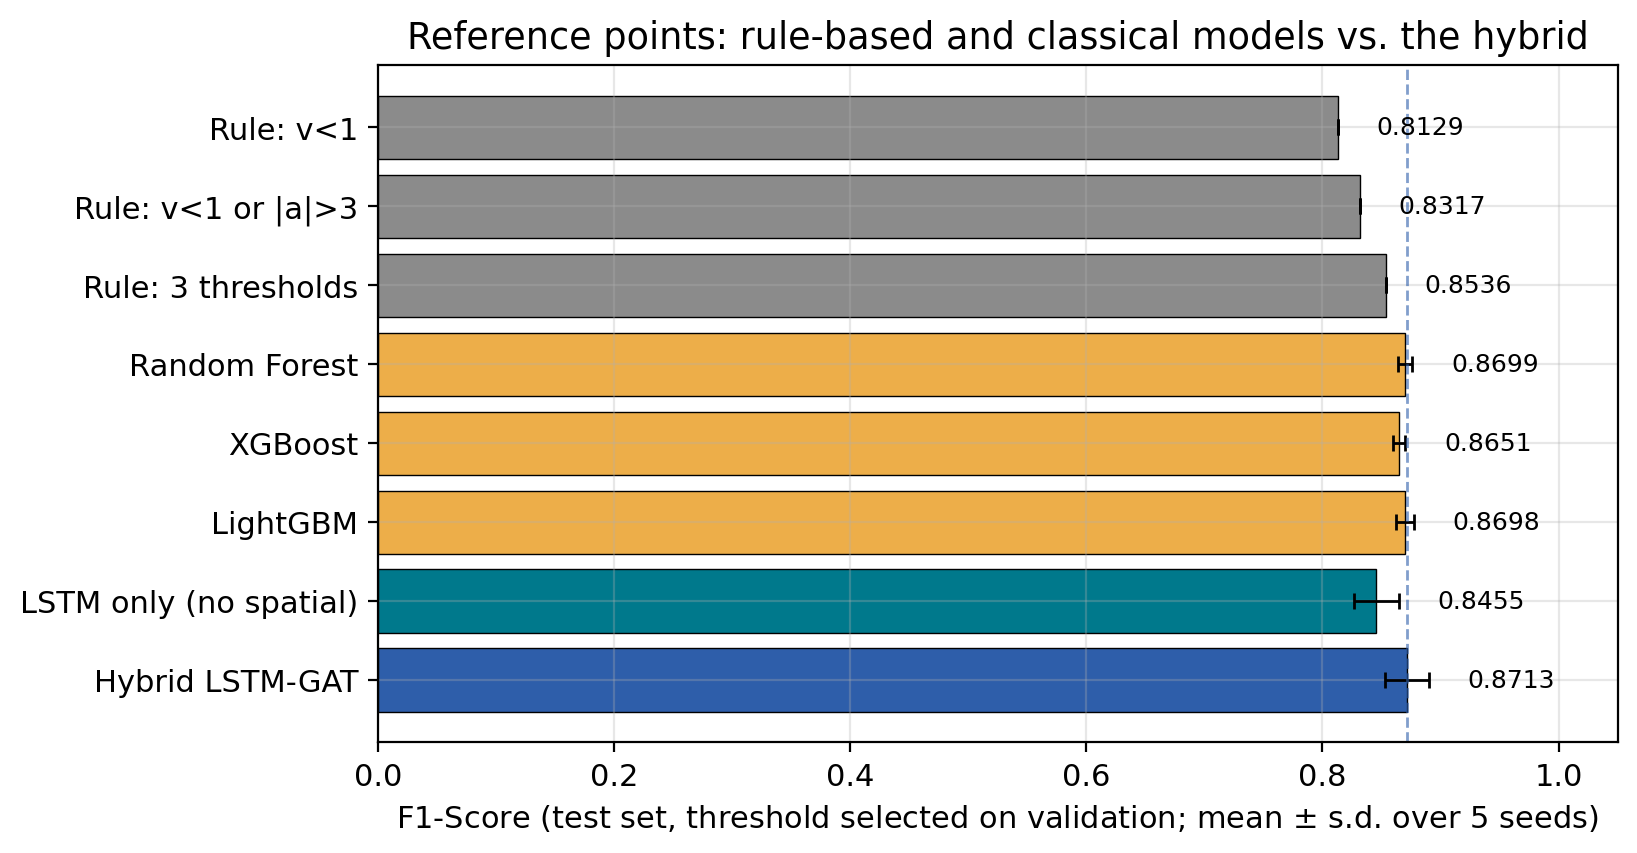
\includegraphics[width=0.95\linewidth]{fig_F1_baselines.png}
  \caption{Reference points: zero-parameter rules and classical feature-based models against the hybrid neural model on the fixed test partition.}
  \label{fig:reference_points}
\end{figure}

\subsection{Encoder Benchmark}
\label{sec:encoder_benchmark}

Reviewers of spatio-temporal anomaly detectors reasonably ask for comparison against STGCN \cite{yu_spatio-temporal_2018}, DCRNN \cite{li_diffusion_2018}, and Graph WaveNet \cite{wu_graph_2019}. These architectures target a structurally different formulation: every graph node carries a continuous time series and the model predicts jointly across all nodes at each step. The present task maps a single vehicle's 50-step window to a single road segment for binary classification, so these models cannot be deployed unmodified.

We therefore isolate the \textbf{core operator} of each architecture and evaluate it under an identical task, budget, partition, fusion operator, and classification head. On the temporal axis we compare the stacked LSTM against a GRU (the DCRNN recurrent backbone), a gated temporal convolution (STGCN), a dilated causal convolution stack with residual and skip connections (Graph WaveNet), and a Transformer encoder. On the spatial axis we compare the GAT against Chebyshev graph convolution (STGCN), bidirectional diffusion convolution (DCRNN), a learnable adaptive adjacency (Graph WaveNet), and no spatial branch at all. This adaptation is a deliberate scoping decision and is stated as such.

Table~\ref{tab:encoder_benchmark} and Fig.~\ref{fig:encoder_benchmark} report the outcome. The fusion operator is held at static weighted summation throughout this benchmark. This choice follows from Section~\ref{sec:fusion_ablation}: the gated operator exhibits a collapse mode that would inject variance unrelated to encoder quality.

\begin{table}[!htbp]
  \centering
  \caption{\textbf{[Fixed partition, 5 seeds, window-level tests]}~ Encoder benchmark, five seeds, identical protocol. The $p$-values are paired McNemar tests against the LSTM--GAT row; Table~\ref{tab:trip_level} repeats them at the trip level.}
  \label{tab:encoder_benchmark}
  \renewcommand{\arraystretch}{1.2}
  \resizebox{\columnwidth}{!}{%
    \begin{tabular}{@{}llccr c@{}}
      \toprule
      \textbf{Config} & \textbf{Origin} & \textbf{F1-Score} & \textbf{ROC-AUC} & \textbf{Params} & \textbf{$p$} \\ \midrule
      \textbf{LSTM + GAT} & \textbf{this study} & $\bm{0.8713 \pm 0.0188}$ & $0.9638$ & 220{,}802 & --- \\
      GRU & DCRNN backbone & $0.8701 \pm 0.0102$ & $\bm{0.9929}$ & 170{,}626 & 0.118 \\
      Transformer & Transformer & $0.8698 \pm 0.0081$ & $0.9899$ & 292{,}098 & 0.815 \\
      Dilated causal conv & Graph WaveNet & $0.8535 \pm 0.0114$ & $0.9799$ & 416{,}258 & 0.115 \\
      No spatial branch & control & $0.8455 \pm 0.0190$ & $0.9294$ & 215{,}234 & 0.549 \\
      Gated TCN & STGCN & $0.8314 \pm 0.0058$ & $0.9861$ & 122{,}242 & \textbf{0.003} \\
      Chebyshev conv & STGCN & $0.8234 \pm 0.0389$ & $0.9481$ & 223{,}106 & \textbf{0.007} \\
      Diffusion conv & DCRNN & $0.8181 \pm 0.0450$ & $0.9633$ & 228{,}290 & \textbf{0.003} \\
      Adaptive adjacency & Graph WaveNet & $0.4657 \pm 0.2833$ & $0.7891$ & 321{,}850 & $\bm{<}$\textbf{0.001} \\ \bottomrule
    \end{tabular}}
\end{table}

\begin{figure}[!htbp]
  \centering
  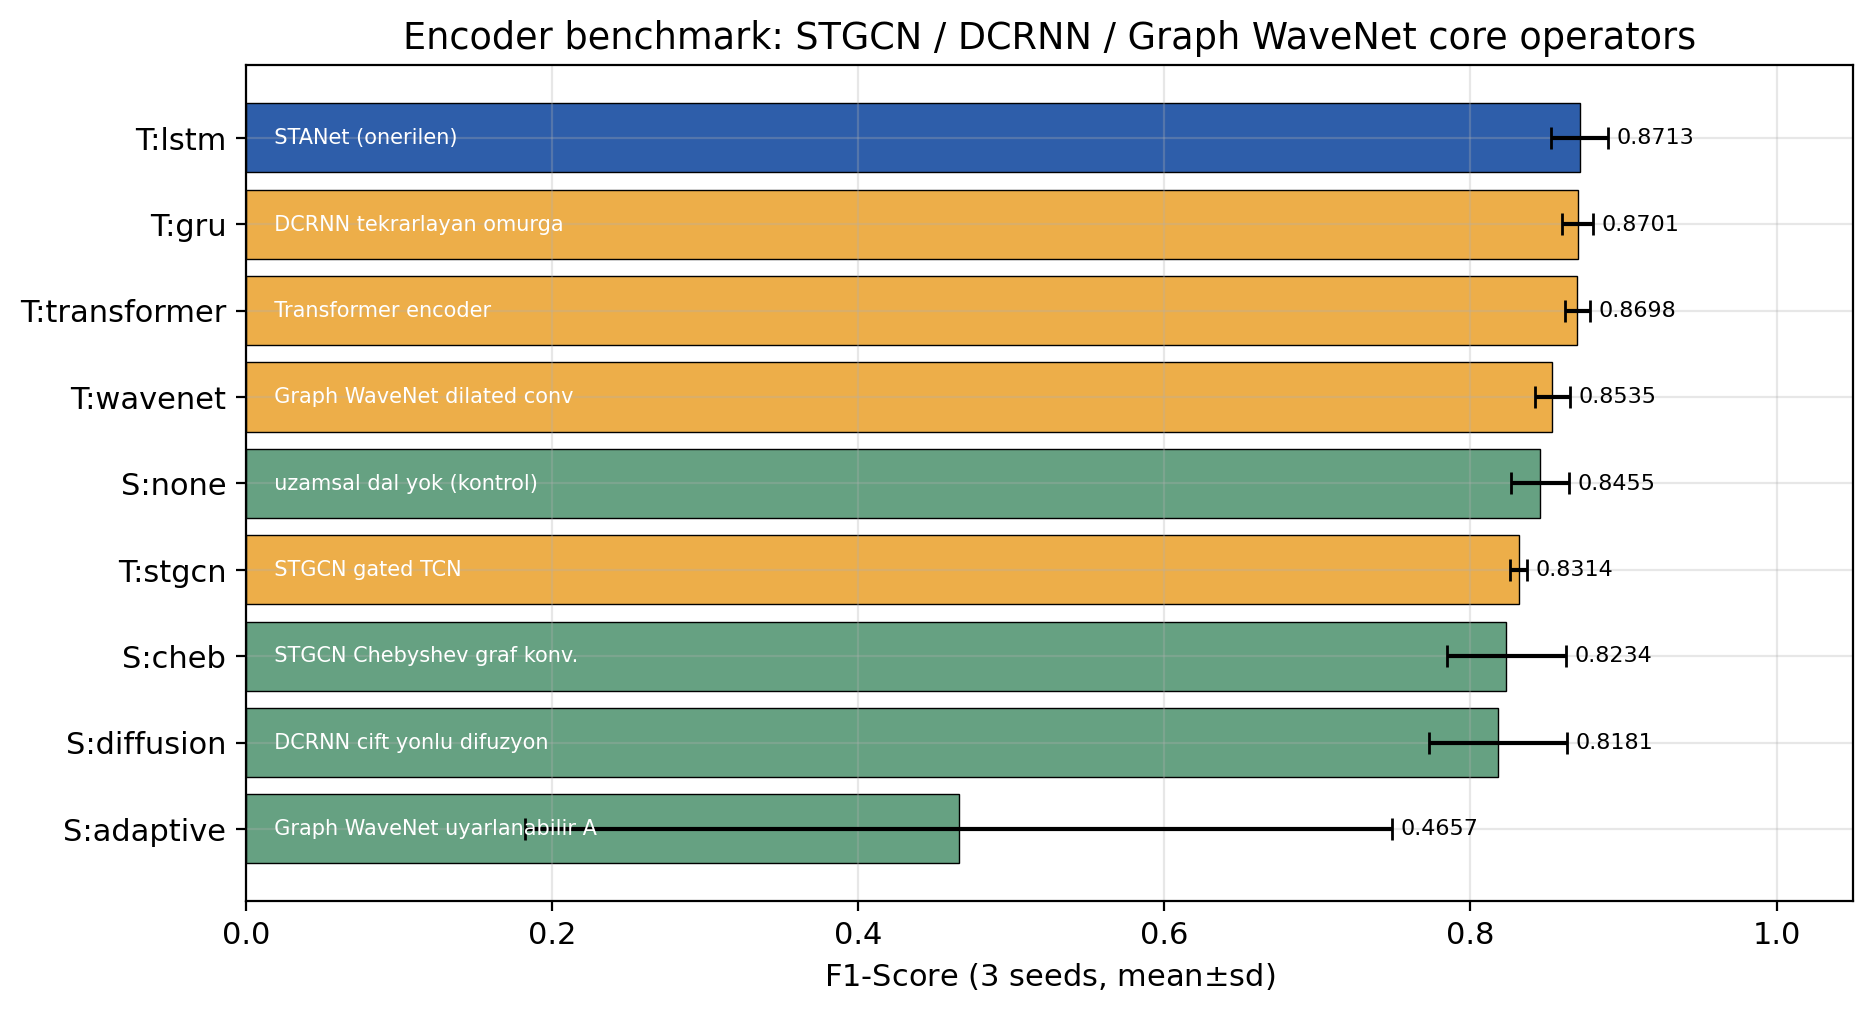
\includegraphics[width=0.98\linewidth]{fig_F4_benchmark.png}
  \caption{Encoder benchmark. Bars show mean F1 over five seeds; error bars show standard deviation.}
  \label{fig:encoder_benchmark}
\end{figure}

The LSTM--GAT pairing attains the highest mean F1 among the nine configurations, but the margin is significant against only four of the eight alternatives, and the identity of those four is the substantive result. The pairing separates cleanly from the STGCN gated temporal convolution ($p = 0.003$) and from all three alternative \emph{spatial} operators---Chebyshev convolution ($p = 0.007$), diffusion convolution ($p = 0.003$), and adaptive adjacency ($p < 0.001$). It does \emph{not} separate from any of the remaining strong temporal encoders: the GRU backbone ($0.8701 \pm 0.0102$, $p = 0.118$), the Transformer encoder ($0.8698 \pm 0.0081$, $p = 0.815$), or the dilated causal convolution stack ($0.8535 \pm 0.0114$, $p = 0.115$). The top three configurations lie within $0.0015$ F1 of one another, an order of magnitude below the leader's own seed standard deviation.

We draw the conclusion the measurement supports rather than the one the architecture was proposed to demonstrate: \textbf{the choice of temporal encoder is not resolvable on this data, while the choice of spatial operator is}. Attention-based aggregation is measurably better than the Chebyshev, diffusion, and adaptive alternatives; whether the recurrence is an LSTM, a GRU, or self-attention is not something these experiments can decide. The GRU reaches the same F1 with $23\%$ fewer parameters and the highest ROC-AUC of any neural configuration, and would be the preferable choice on that basis alone.

Two negative results are informative. Replacing the GAT with Chebyshev or diffusion convolution falls \emph{below} the no-spatial-branch control, indicating that graph message passing is not intrinsically helpful here and that any benefit is specific to attention-based aggregation. More strikingly, Graph WaveNet's learnable adaptive adjacency collapses ($0.4657 \pm 0.2833$): parameterizing a free $4{,}678 \times 4{,}678$ adjacency matrix is not identifiable at this data scale. Together with Section~\ref{sec:fusion_ablation}, a consistent pattern emerges---\textbf{freely parameterized adaptive components are unstable in this regime, whereas fixed or minimally parameterized alternatives are both stronger and more reliable}.

\paragraph{Note on the previous version} The margins reported here are smaller and fewer than in the earlier version of this work, which reported $0.8836 \pm 0.0033$ for LSTM--GAT and significance against the DCRNN backbone and both Graph WaveNet components. That table was computed over three seeds rather than five. Extending to five seeds raised the leader's standard deviation from $0.0033$ to $0.0188$, and the comparisons against the GRU and dilated-convolution encoders ceased to be significant. A three-seed standard deviation of $0.0033$ on a configuration whose five-seed spread is $0.0188$ is not a small error bar; it is an under-sampled one.

\subsection{Fusion Ablation}
\label{sec:fusion_ablation}

We now hold both encoders fixed and vary only the fusion operator, over five seeds. Table~\ref{tab:fusion_ablation} and Fig.~\ref{fig:fusion_ablation} summarize the outcome.

\begin{table}[!htbp]
  \centering
  \caption{\textbf{[Fixed partition, 5 seeds]}~ Fusion ablation, five seeds, all other components identical}
  \label{tab:fusion_ablation}
  \renewcommand{\arraystretch}{1.2}
  \resizebox{\columnwidth}{!}{%
    \begin{tabular}{@{}lcccr@{}}
      \toprule
      \textbf{Fusion} & \textbf{F1-Score} & \textbf{ROC-AUC} & \textbf{Worst seed} & \textbf{Params} \\ \midrule
      \textbf{Static weighted sum} & $\bm{0.8713 \pm 0.0188}$ & $\bm{0.9638}$ & $0.8491$ & \textbf{1} \\
      Cross-attention & $0.8559 \pm 0.0228$ & $0.9417$ & $0.8369$ & 16{,}640 \\
      Fixed concatenation & $0.8442 \pm 0.0091$ & $0.8993$ & $0.8339$ & 0 \\
      Gated (proposed) & $0.6953 \pm 0.3488$ & $0.8752$ & $\bm{0.0715}$ & 4{,}161 \\ \bottomrule
    \end{tabular}}
\end{table}

\begin{figure}[!htbp]
  \centering
  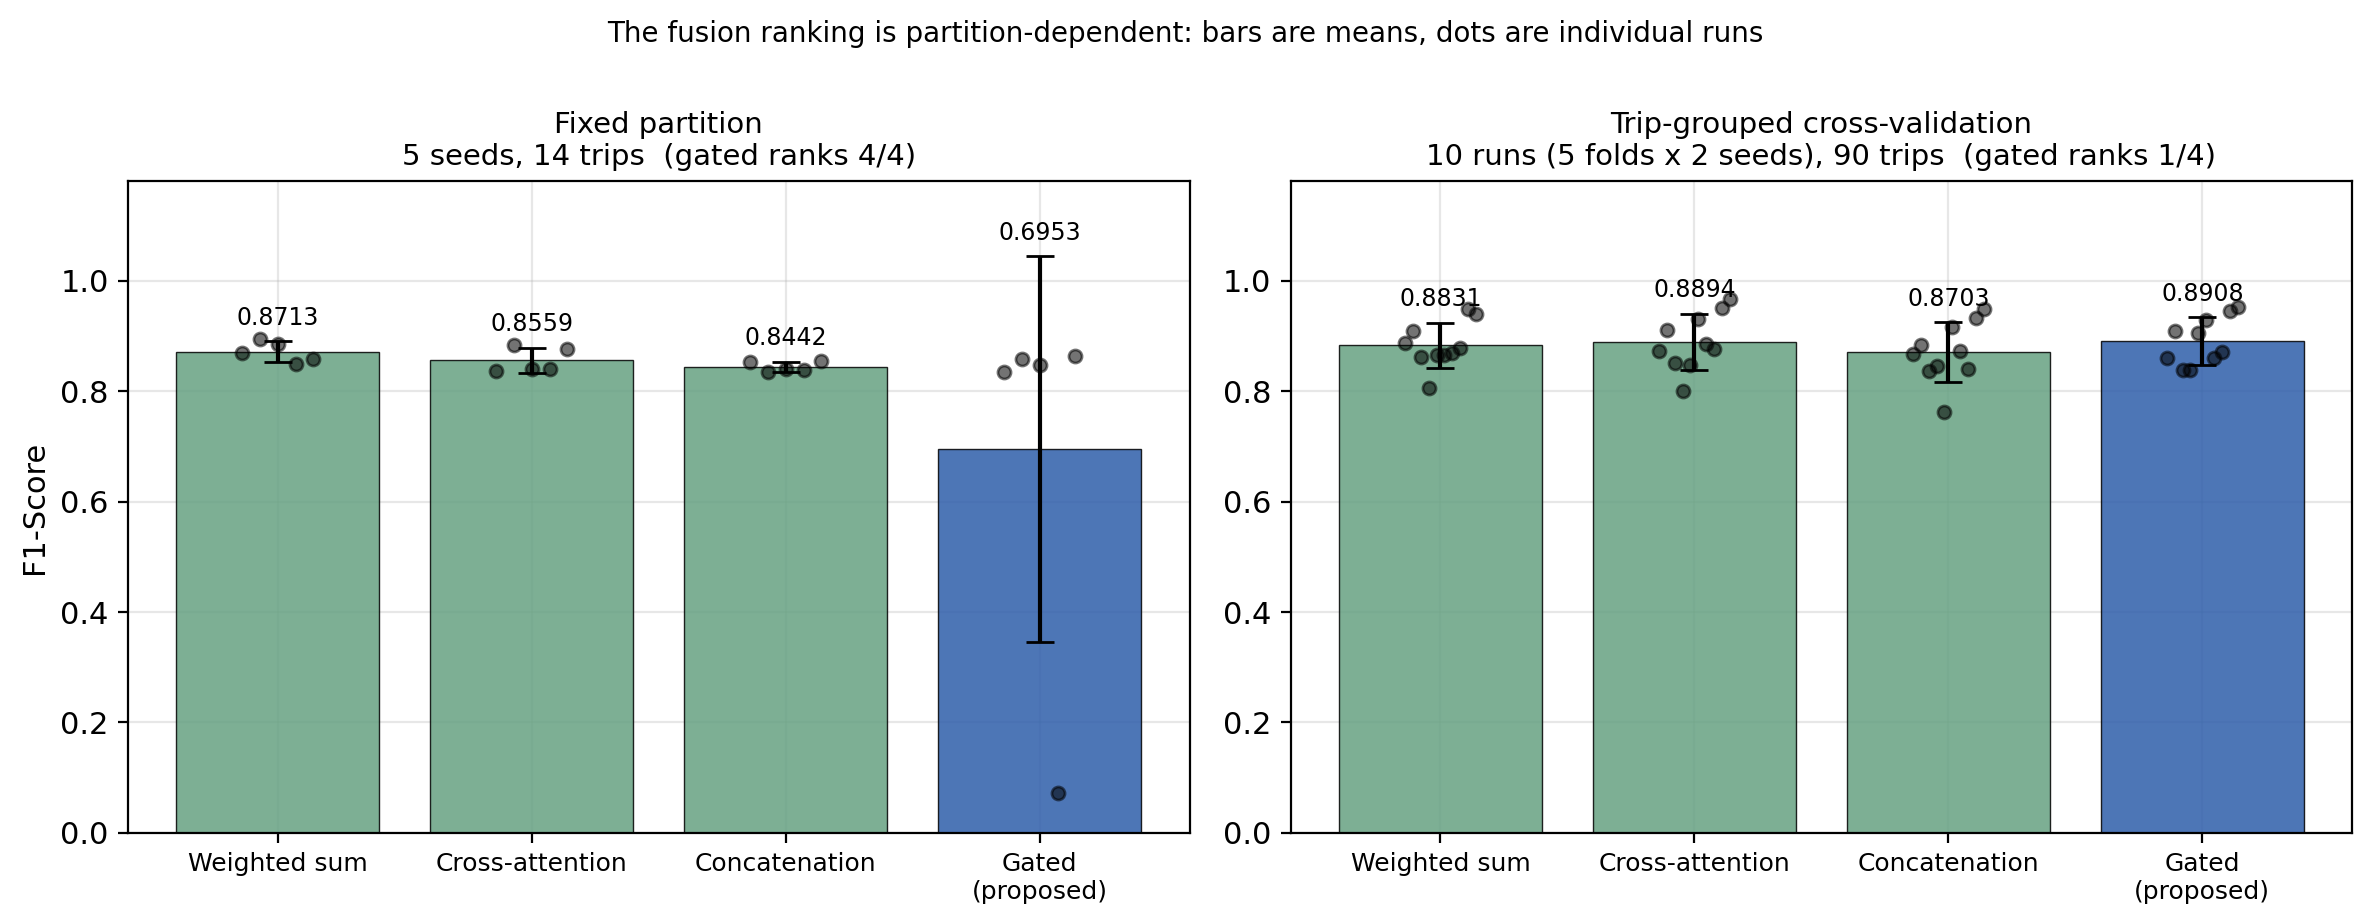
\includegraphics[width=0.98\linewidth]{fig_F3_fusion_ablation.png}
  \caption{The fusion ranking is partition-dependent. Left: the fixed partition (five seeds, 14 trips), where the gated operator ranks fourth of four and one run collapses. Right: trip-grouped cross-validation (ten runs, 90 trips), where the same operator ranks first of four and no run collapses. Bars are means with standard deviation; dots are individual runs. Under cross-validation no pairwise difference is significant at the trip level after Holm correction (Section~\ref{sec:cv}).}
  \label{fig:fusion_ablation}
\end{figure}

The sample-wise gate ranks \textbf{last of four}. Two aspects of this result matter more than the ranking itself.

\textbf{A degenerate collapse mode.} In one of five seeds the gated model failed completely ($\mathrm{F1}=0.0715$), with a mean $g_{gate}$ of $0.026$ and a mean of $0.0125$ on anomalous samples. The gate had locked onto the spatial modality, which---as Section~\ref{sec:encoder_benchmark} shows---cannot classify on its own, and training could not escape. Equation~\ref{eq:gated_fusion} admits this optimum by construction: as $g_{gate}\rightarrow 0$ the temporal signal is suppressed multiplicatively and its gradient vanishes with it. Concatenation has no such mode, because the classifier weights the two embeddings independently and can simply ignore the uninformative one. No collapse occurred in any of the fifteen runs of the other three operators.

This collapse is reproducible in the strongest sense available to us. The earlier version of this study observed it at seed $45$ under a different cuDNN configuration ($\mathrm{F1}=0.0833$). The experiments reported here were re-run from scratch under the protocol of Section~\ref{sec:protocol_note}, and the collapse recurred \emph{at the same seed} with a comparable magnitude. It is a property of the operator and this initialization, not an artifact of a particular backend setting.

\textbf{The learned optimum is a constant.} In the static weighted-sum variant, the single learnable scalar converged to $\{0.519, 0.522, 0.518, 0.498, 0.497\}$ across the five seeds---that is, to approximately equal weighting in every run. The data does not call for a sample-dependent mixing weight. A one-parameter static weight outperforms the $4{,}161$-parameter adaptive gate, and does so with an order of magnitude lower seed variance ($\pm 0.0188$ versus $\pm 0.3488$).

Paired single-run tests are the wrong instrument for this comparison. On the median seed the gated model is indistinguishable from concatenation ($p = 1.000$) and from cross-attention ($p = 0.727$), and its difference from the static weighted sum is $-0.0379$ with interval $[-0.0708, -0.0119]$; none of these single-partition numbers reflects the $0.35$ standard deviation that is the substantive finding. Across-seed instability is not visible to a test that examines one seed. This is itself an argument for the multi-seed protocol of Section~\ref{sec:repeatability}.

\begin{table}[!htbp]
  \centering
  \caption{\textbf{[Fixed partition, 5 seeds]}~ Cost of the four fusion operators. Fusion parameters counts only the operator; total counts the whole model. Epochs and training time are means over the five fixed-partition seeds, on one NVIDIA RTX 4060 Laptop GPU. Latency is the median over a single window, measured on the trip-instance graph.}
  \label{tab:fusion_cost}
  \renewcommand{\arraystretch}{1.15}
  \resizebox{\columnwidth}{!}{%
    \begin{tabular}{@{}lrrccccc@{}}
      \toprule
      \textbf{Fusion} & \textbf{Fusion par.} & \textbf{Total par.} & \textbf{Epochs} & \textbf{Train (min)} & \textbf{GPU (ms)} & \textbf{GPU cached} & \textbf{CPU (ms)} \\ \midrule
      Static weighted sum & 1 & 220{,}802 & $34.4$ & $2.72$ & $2.87$ & $0.64$ & $27.82$ \\
      Fixed concatenation & 0 & 222{,}849 & $19.8$ & $1.50$ & $2.56$ & $0.55$ & $23.14$ \\
      Sample-wise gate & 4{,}161 & 224{,}962 & $31.4$ & $2.66$ & $2.80$ & $0.78$ & $25.07$ \\
      Cross-attention & 16{,}640 & 237{,}441 & $30.0$ & $2.49$ & $2.91$ & $0.96$ & $19.83$ \\ \bottomrule
    \end{tabular}}
\end{table}

Table~\ref{tab:fusion_cost} answers a question the ranking alone leaves open: what the four operators cost. The span in fusion parameters is four orders of magnitude, from none at all for concatenation to $16{,}640$ for cross-attention, yet total model size varies by under $8\%$ because the temporal branch dominates. Training time and single-window latency differ by less than the seed-to-seed variation in either. Cross-attention is the most expensive operator on every axis and finishes second of four under cross-validation and second on the fixed partition; the single scalar of the weighted sum is the cheapest learnable option and finishes third and first respectively. Neither ordering is significant (Section~\ref{sec:cv}), which is the point: the operators differ in cost far more than the measurements can distinguish them in accuracy.

\subsection{Gate Behavior}
\label{sec:gate_behaviour}

Section~\ref{sec:fusion_module} established that gating can only outperform concatenation through genuinely sample-dependent behavior. Fig.~\ref{fig:gate} examines whether such behavior is observed, by measuring the class-conditional shift $\bar{g}_{\text{anomalous}} - \bar{g}_{\text{normal}}$ across seeds.

\begin{figure}[!htbp]
  \centering
  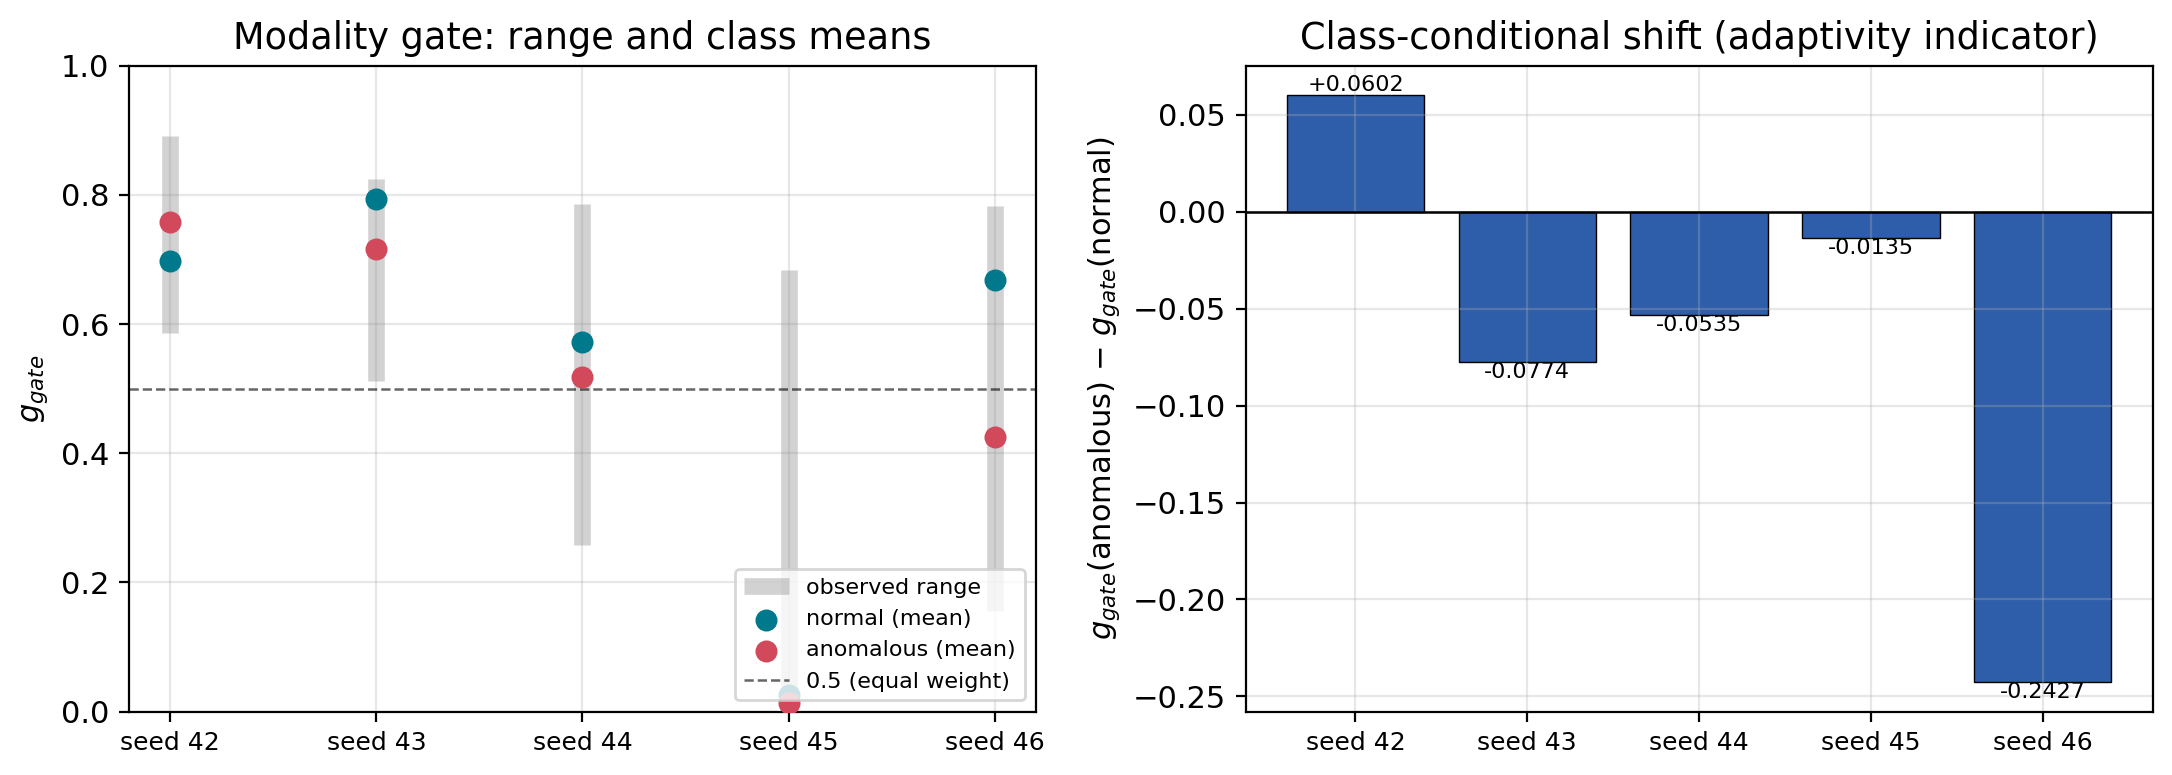
\includegraphics[width=0.98\linewidth]{fig_F3_gate.png}
  \caption{Modality gate behavior across five seeds. Left: observed range and class means. Right: class-conditional shift, which is inconsistent in both magnitude and sign.}
  \label{fig:gate}
\end{figure}

The measured shifts are $+0.0602$, $-0.0774$, $-0.0535$, $-0.0135$, and $-0.2427$. Both the magnitude and the \emph{sign} vary across seeds. A class-conditional interpretation of the gate---for instance, that anomalous samples shift weight toward the temporal branch---is therefore not a stable property of the trained model but an observation that holds in one run and reverses in the other four.

This is a correction to the interpretation offered in the earlier version of this work, which reported a shift from $0.70$--$0.75$ on normal samples to approximately $0.80$ on anomalous samples based on a single checkpoint. Re-evaluating the archived checkpoint gives class means of $0.860$ and $0.856$ respectively---a difference of $0.004$, with the gate never falling below $0.5$ on any sample. We report this explicitly because interpretability claims derived from one training run are exactly the kind of evidence this study argues against.

\subsection{Cross-Validated Evaluation and Subtype Stratification}
\label{sec:cv}

The fixed partition of Table~\ref{tab:dataset_split} contains 157 positive test instances drawn from 14 trips. Section~\ref{sec:trip_level} showed that this supports no inferential claim. We therefore repeat the entire evaluation---all four fusion operators and the spatial-branch control---under five-fold trip-grouped cross-validation crossed with two seeds, giving ten runs per configuration. Every sequence receives an out-of-fold test prediction, so all \textbf{90 trips} enter the analysis rather than 14, and fold-wise test prevalence ranges from $3.40\%$ to $10.49\%$. This is the primary evidence base of the paper.

\begin{table}[!htbp]
  \centering
  \caption{\textbf{[Cross-validation, 5 folds $\times$ 2 seeds]}~ Five-fold trip-grouped cross-validation crossed with two seeds (ten runs per configuration, all 28{,}090 sequences). Collapse counts runs with $\mathrm{F1} < 0.30$.}
  \label{tab:cv}
  \renewcommand{\arraystretch}{1.2}
  \resizebox{\columnwidth}{!}{%
    \begin{tabular}{@{}lcccccc@{}}
      \toprule
      \textbf{Model} & \textbf{Run F1} & \textbf{Worst} & \textbf{Collapse} & \textbf{Pooled F1} & \textbf{Brier} & \textbf{ECE} \\ \midrule
      Gated hybrid & $\bm{0.8908 \pm 0.0429}$ & $\bm{0.8385}$ & 0/10 & $0.8849$ & $0.0257$ & $0.0579$ \\
      Cross-attention hybrid & $0.8894 \pm 0.0510$ & $0.8007$ & 0/10 & $0.8838$ & $0.0267$ & $0.0627$ \\
      LSTM only (control) & $0.8839 \pm 0.0436$ & $0.8302$ & 0/10 & $\bm{0.8901}$ & $\bm{0.0208}$ & $0.0548$ \\
      Weighted-sum hybrid & $0.8831 \pm 0.0412$ & $0.8062$ & 0/10 & $0.8891$ & $0.0236$ & $\bm{0.0409}$ \\
      Concatenation hybrid & $0.8703 \pm 0.0543$ & $0.7621$ & 0/10 & $0.8528$ & $0.0254$ & $0.0560$ \\ \bottomrule
    \end{tabular}}
\end{table}

\textbf{The fusion ranking reverses.} On the fixed partition the gated operator finished last of four and collapsed in one of five seeds; across five trip partitions it finishes \emph{first} of four and collapses in none of ten runs. Its worst cross-validated run is $0.8385$, against $0.0715$ on the fixed partition. The concatenation operator, third on the fixed partition, is last here.

Neither ordering should be reported as a result, and we report neither. At the trip level, gating differs from the weighted sum by $-0.0042$ ($95\%$ CI $[-0.0162, +0.0102]$, Holm $p = 1.000$), from cross-attention by $+0.0011$ ($95\%$ CI $[-0.0120, +0.0175]$, Holm $p = 1.000$), and from concatenation by $+0.0321$ ($95\%$ CI $[+0.0052, +0.0689]$, Holm $p = 0.099$). \textbf{No fusion operator is distinguishable from any other} once the correct unit and multiplicity correction are applied. The four configurations span $0.0205$ F1, against a within-configuration standard deviation of $0.04$--$0.05$.

The comparison against concatenation is the closest to significance (uncorrected $p = 0.033$), and it is also the one most affected by the pooling correction of Section~\ref{sec:protocol_note}: concatenation's pooled F1 falls by $0.0244$ when each run is scored at its own threshold, more than any other variant. We note this rather than resting on it.

This is the paper's central empirical statement, and it cuts in both directions. It does not vindicate the sample-wise gate: nothing here shows the gate helping. It equally does not condemn it: the fixed-partition result that placed it last, including its collapse, is not reproduced when five partitions are used instead of one. \textbf{What the data supports is that the choice of fusion operator in this setting is not resolvable}---and that a study reporting a ranking from a single partition, as the earlier version of this work did, would have reported one of two opposite orderings depending on which partition it happened to use.

The collapse mode of Section~\ref{sec:fusion_ablation} remains a real and reproducible phenomenon; it recurred at the same seed across a full re-run under a different backend configuration. What these ten cross-validated runs establish is that it is \emph{rare} rather than systematic, and Section~\ref{sec:graph_ablation} shows it is conditional on the spatial branch being nearly uninformative. A failure mode that appears in one of fifteen runs is worth documenting for practitioners; it is not evidence that one operator is generally worse than another.

The spatial-branch control is equally instructive: removing the spatial branch entirely yields $0.8839 \pm 0.0436$, statistically indistinguishable from every hybrid variant. On the fixed partition the same ablation appeared to cost $3.5$ F1 points
at $p = 0.035$.  % ESKI-DEGER: geri cekilen v1 iddiasi, bilerek aniliyor
We \textbf{withdraw that claim}. Section~\ref{sec:subtype} examines whether the spatial branch helps anywhere at all.

\subsubsection{Subtype Stratification}
\label{sec:subtype}
Section~\ref{sec:reference_points} identified speed-limit violation as the one anomaly subtype whose defining rule depends on a quantity ($v_{\max}$) available only to the spatial branch. Pooling out-of-fold predictions gives 144 such sequences drawn from all 90 trips---enough for a stratified comparison that the single partition, with 13 positives from 14 trips, could not support. Table~\ref{tab:subtype} and Fig.~\ref{fig:subtype} report the result, with all tests at the trip level and Holm correction across the three subtypes.

\begin{table*}[!t]
  \centering
  \caption{\textbf{[Cross-validation, pooled, trip-level tests]}~ All anomaly subtypes present in the data, on pooled cross-validated predictions. Windows counts positive windows; Trips counts the trips containing at least one. Precision, recall and F1 are for the hybrid with weighted-sum fusion; the final columns compare it against the control without a spatial branch. Intervals and $p$-values are trip-level over the 90 trips and are reported only where the subtype has at least 5 positive trips and 30 positive windows; rows marked $\dagger$ are below that and are given descriptively. False positives are shared across rows: the negative set is held fixed and only the positive subset changes, so the hybrid records 89 false positives against every subtype and differences in F1 arise from recall. Subtype 6 of the taxonomy (GPS speed artefact) does not occur in the generated data.}
  \label{tab:subtype}
  \renewcommand{\arraystretch}{1.15}
  \resizebox{\textwidth}{!}{%
    \begin{tabular}{@{}lrrccccccc@{}}
      \toprule
      \textbf{Subtype} & \textbf{Windows} & \textbf{Trips} & \textbf{Precision} & \textbf{Recall} & \textbf{F1} & \textbf{LSTM-only F1} & \textbf{$\Delta$} & \textbf{Trip 95\% CI} & \textbf{$p$} \\ \midrule
      Abnormal dwell & 1{,}154 & 33 & $0.9250$ & $0.9515$ & $0.9381$ & $0.9307$ & $+0.0074$ & $[-0.0080, +0.0265]$ & 0.406 \\
      Crash & 569 & 7 & $0.8578$ & $0.9438$ & $0.8987$ & $0.8935$ & $+0.0052$ & $[-0.0519, +0.1054]$ & 0.852 \\
      Speed-limit violation & 144 & 28 & $0.1759$ & $0.1319$ & $0.1508$ & $0.2288$ & $-0.0780$ & $[-0.3044, +0.1152]$ & 0.506 \\
      Signal freeze & 62 & 24 & $0.0220$ & $0.0323$ & $0.0261$ & $0.0848$ & $-0.0587$ & $[-0.1283, -0.0046]$ & 0.043 \\
      Abnormal heading change$^{\dagger}$ & 21 & 13 & $0.0220$ & $0.0952$ & $0.0357$ & $0.0336$ & $+0.0021$ & --- & --- \\
      Abnormal acceleration$^{\dagger}$ & 19 & 15 & $0.0111$ & $0.0526$ & $0.0183$ & $0.0342$ & $-0.0158$ & --- & --- \\
      GPS acceleration artefact$^{\dagger}$ & 8 & 8 & $0.0111$ & $0.1250$ & $0.0204$ & $0.0377$ & $-0.0173$ & --- & --- \\
      GPS heading artefact$^{\dagger}$ & 8 & 6 & $0.0000$ & $0.0000$ & $0.0000$ & $0.0000$ & $+0.0000$ & --- & --- \\ \bottomrule
    \end{tabular}}
\end{table*}

\begin{figure}[!htbp]
  \centering
  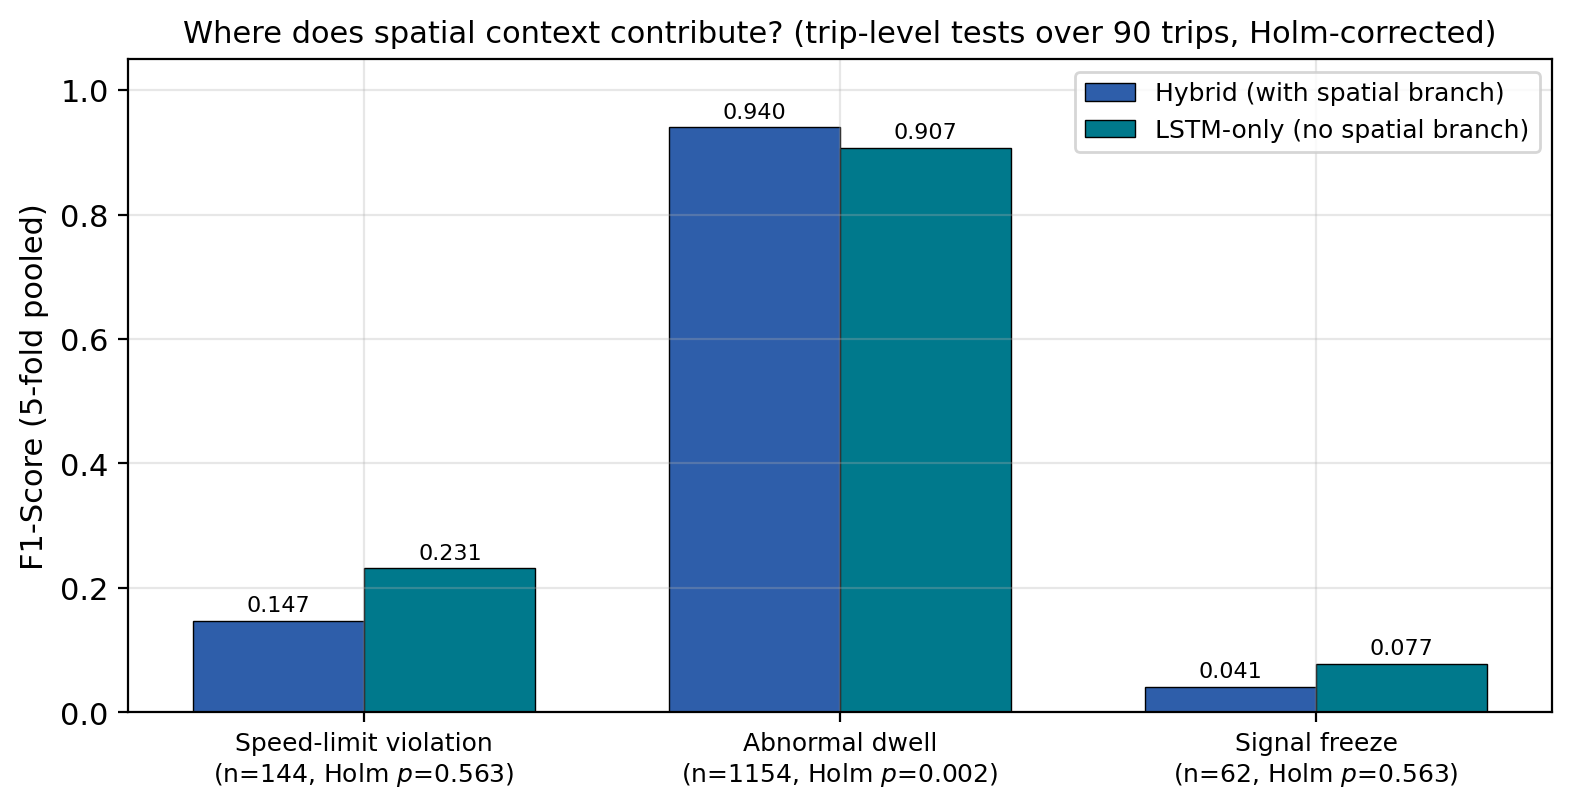
\includegraphics[width=0.95\linewidth]{fig_F5_subtype.png}
  \caption{Subtype stratification on pooled cross-validated predictions. The spatial branch helps where it was not predicted to (abnormal dwell) and does not help where it holds the decisive feature (speed-limit violation).}
  \label{fig:subtype}
\end{figure}

No comparison in this table is significant at the trip level after Holm correction, and the table is worth reading carefully because an earlier version of this work reported one that was.

\textbf{The predicted effect is absent.} On speed-limit violations---the subtype whose generating rule is a function of $v_{\max}$, a quantity present only in the node features---the hybrid model is \emph{worse} than the temporal-only model ($0.1508$ versus $0.2288$), and the interval $[-0.2986, +0.1219]$ spans zero. Both are weak in absolute terms. We verified that the label rule and the model input use the same speed limit: applying the documented rule $v > 1.10\,v_{\max}$ directly to the node feature recovers all 13 positive windows in the fixed test partition. Five of those thirteen lie on segments whose speed limit is an author-defined default, so the circularity noted in Section~\ref{sec:threats} is real and, for this subtype, rests partly on an imputed value. The branch nonetheless fails to exploit the feature.

\textbf{The unpredicted effect has also gone.} Abnormal dwell was reported in the previous version as a gain of $+0.0335$ F1 with a Holm-corrected $p$ of $0.002$, the study's only comparison significant at the trip level. % ESKI-DEGER: geri cekilen v1 iddiasi
It was an artifact of the pooling defect described in Section~\ref{sec:protocol_note}: the pooled analysis applied the mean of all fold-seed thresholds to every prediction rather than each run's own. With each run scored at its own validation threshold the gain is $+0.0074$, with an interval of $[-0.0084, +0.0268]$ that contains zero and a Holm-corrected $p$ of $0.814$. \textbf{We withdraw that finding.}

\textbf{What remains is a hint in the opposite direction.} Signal freeze has an uncorrected trip-level $p$ of $0.0431$ and an interval of $[-0.1238, -0.0065]$ that excludes zero---but the sign is negative: the hybrid is \emph{worse} than the control ($0.0261$ versus $0.0848$). After correction across the three subtypes it is not significant ($0.129$), and with 62 positive windows we do not claim it. We report it because it is now the comparison closest to significance in the study, and reporting only the directions that favour the proposed architecture is the practice this paper argues against.

Across all three subtypes, therefore, \textbf{no evidence remains that the spatial branch contributes to detection}.

\subsection{Effect Sizes and the Distribution Across Trips}
\label{sec:effect_sizes}
A pooled difference is a single number, and a reader is entitled to ask whether it summarises a consistent effect or averages over trips that disagree. Fig.~\ref{fig:per_trip} shows the per-trip differences behind the three comparisons that matter most, and Table~\ref{tab:effect_sizes} gives standardised effect sizes for them.

Two features of the design constrain what this can show. Only $39$ of the $90$ trips contain at least one positive window, so a per-trip F1 is defined for those $39$; the remaining $51$ contribute false positives but no recall, and are reported separately in the result files. The effective sample for any trip-level statement about detection quality is therefore smaller than the trip count alone suggests.

\begin{table}[!htbp]
  \centering
  \caption{\textbf{[Cross-validation, pooled, per-trip]}~ Standardised effect sizes over the 39 trips containing at least one positive window. Cohen's $d$ is computed on the paired per-trip differences. The final column counts trips favouring the first model against the second, with ties omitted.}
  \label{tab:effect_sizes}
  \renewcommand{\arraystretch}{1.15}
  \resizebox{\columnwidth}{!}{%
    \begin{tabular}{@{}lcccc@{}}
      \toprule
      \textbf{Comparison} & \textbf{Mean $\Delta$} & \textbf{s.d.} & \textbf{Cohen's $d$} & \textbf{Trips for / against} \\ \midrule
      Weighted sum vs.\ LSTM only & $-0.0092$ & $0.0885$ & $-0.10$ & 18 / 14 \\
      Gated vs.\ LSTM only & $-0.0146$ & $0.0899$ & $-0.16$ & 15 / 16 \\
      Gated vs.\ weighted sum & $-0.0054$ & $0.0330$ & $-0.16$ & 12 / 18 \\ \bottomrule
    \end{tabular}}
\end{table}

\begin{figure*}[!t]
  \centering
  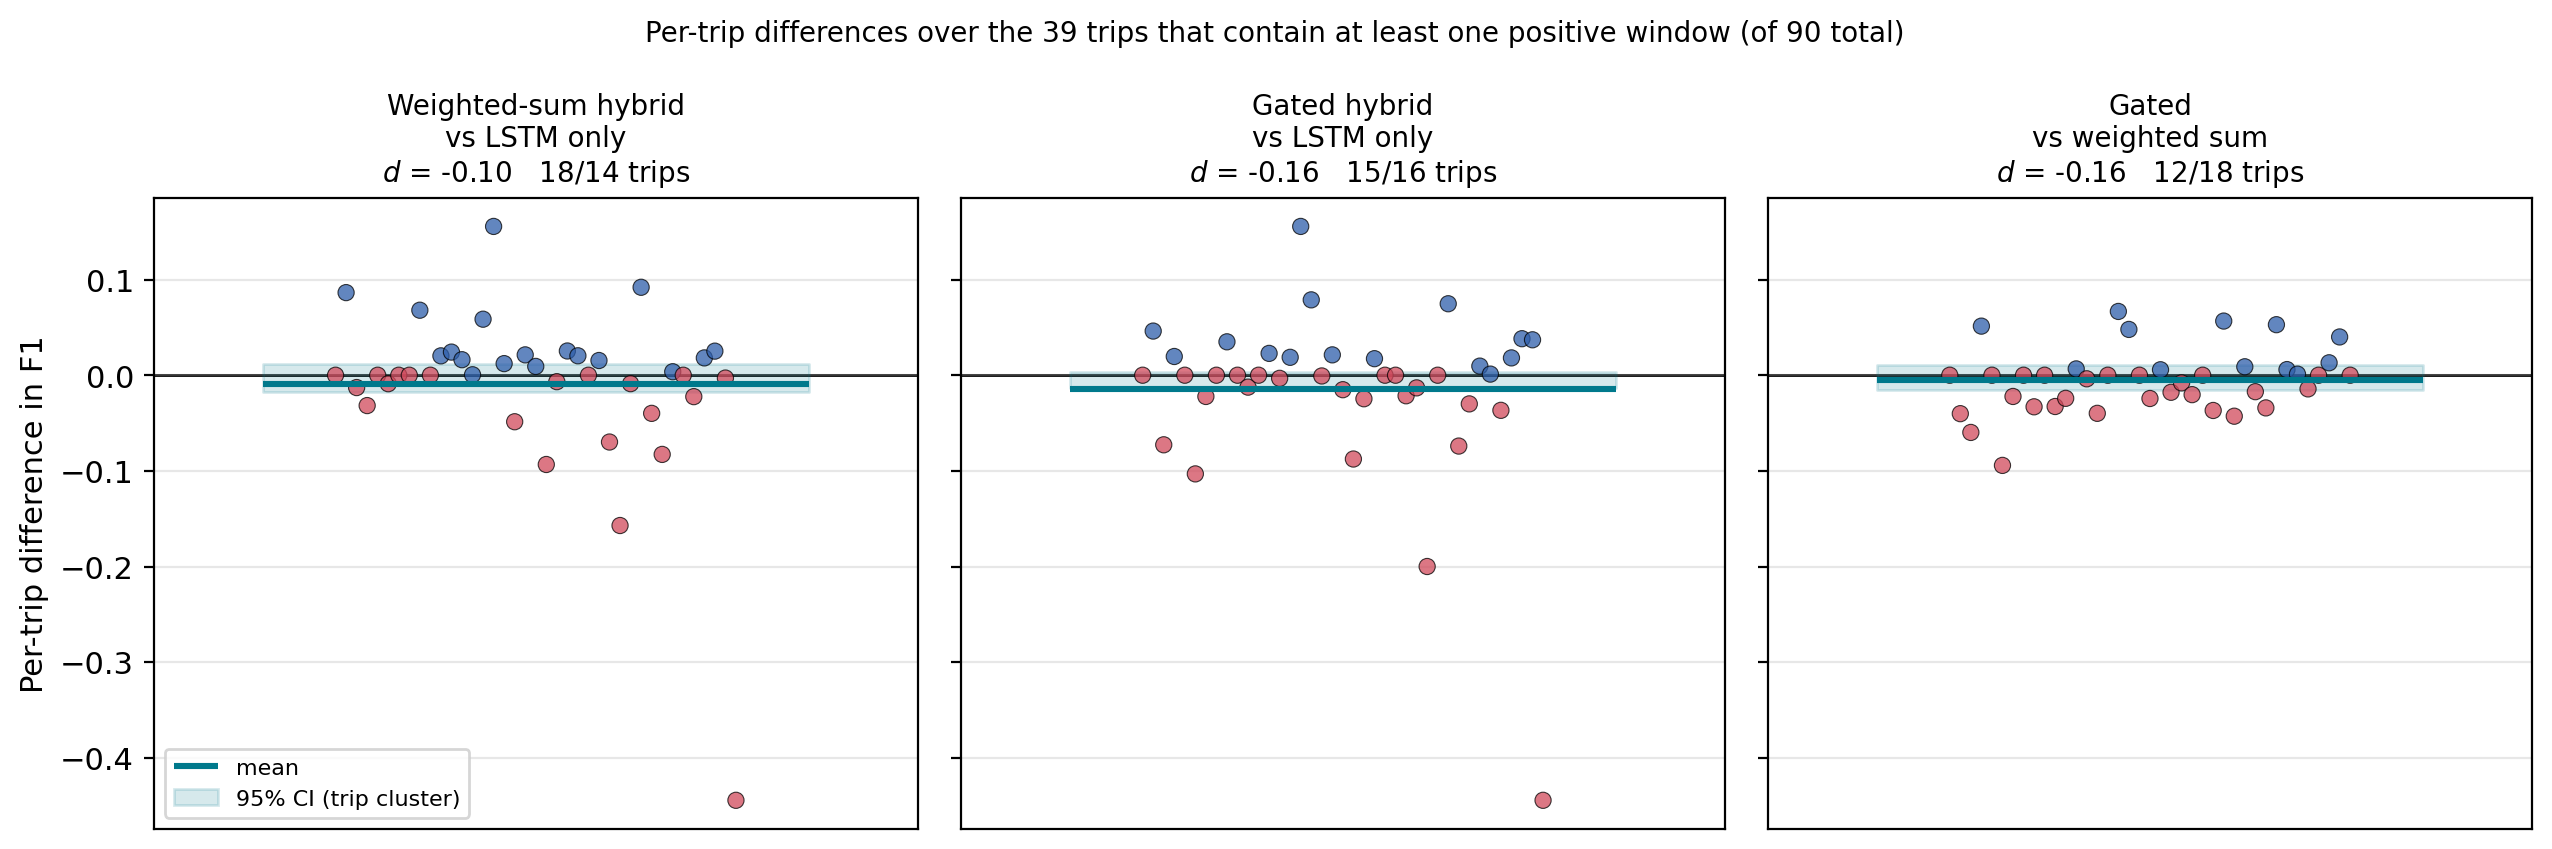
\includegraphics[width=0.95\textwidth]{fig_F8_per_trip.png}
  \caption{Per-trip differences in F1 for the three principal comparisons, over the 39 trips that contain at least one positive window. Each point is one trip; the horizontal band is the trip-level cluster-bootstrap interval for the pooled difference. The differences are centred near zero with trips falling on both sides, and each comparison has one trip whose difference is an order of magnitude larger than the rest.}
  \label{fig:per_trip}
\end{figure*}

All three effect sizes are small by any conventional reading: $|d| \leq 0.16$. More informative than the magnitude is the split. For the weighted-sum hybrid against the temporal-only control, 18 trips favour the hybrid and 14 favour the control, with 7 tied. A pooled mean of $-0.0092$ is not a small consistent advantage; it is the average of a distribution straddling zero. The single trip at $-0.4444$ contributes more to that mean than the median trip does, which is the behaviour the trip-level resampling of Section~\ref{sec:statistical_unit} is designed to account for.

\subsection{Calibration}
\label{sec:calibration}
Probability calibration was not assessed in the previous version of this work. Table~\ref{tab:cv} and the reliability diagram in Fig.~\ref{fig:calibration} report it. The best-calibrated hybrid is the weighted-sum variant (ECE $0.0409$), ahead of concatenation ($0.0560$), gating ($0.0579$), and cross-attention ($0.0627$); the temporal-only control attains the lowest Brier score ($0.0208$).

We note this as a correction to the earlier version of this work, which reported the gated operator as clearly best calibrated (ECE $0.0338$ against $0.0594$ for the weighted sum) on the basis of a single seed per fold. With two seeds per fold the ordering of the two is reversed and the gap is small. Calibration differences of this magnitude are not separable from run-to-run variation at this sample size, and we no longer claim calibration as an advantage of the gating mechanism.

\begin{figure}[!htbp]
  \centering
  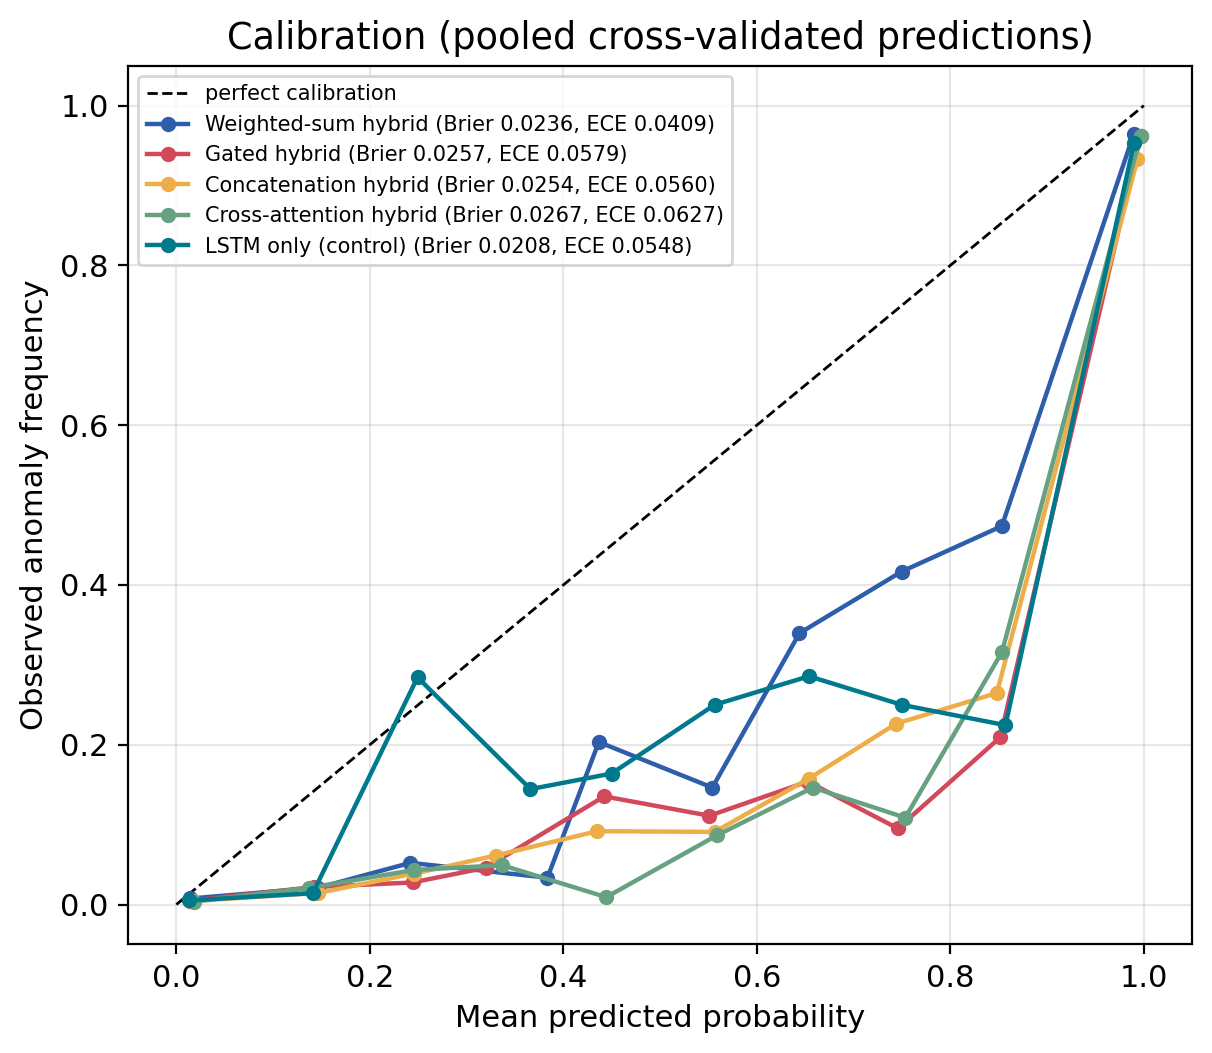
\includegraphics[width=0.75\linewidth]{fig_F5_calibration.png}
  \caption{Reliability diagram from pooled cross-validated predictions.}
  \label{fig:calibration}
\end{figure}

The general point survives the correction even though the specific claim does not. In a monitoring context where alerts are ranked or thresholded by predicted risk, a better-calibrated score is more useful than a marginally higher F1, and calibration is worth reporting for that reason regardless of which variant wins. All five configurations are mildly overconfident, with ECE between $0.041$ and $0.063$; none is well enough calibrated to be used as a risk score without post-hoc recalibration.

\subsection{Graph Construction Ablation}
\label{sec:graph_ablation}
Section~\ref{sec:graph_construction} noted that the graph can be built from trip-specific segment instances ($4{,}678$ nodes) or merged by physical road ($628$ nodes). Table~\ref{tab:graph_ablation} reports both.

\begin{table}[!htbp]
  \centering
  \caption{\textbf{[Fixed partition, 5 seeds]}~ Effect of graph construction, five seeds. The fusion operator is
  named explicitly in every row: an earlier version of this table labelled its
  hybrid rows only as ``hybrid'', which made them appear inconsistent with the
  fusion ablation of Table~\ref{tab:fusion_ablation} when in fact a different
  operator had been used.}
  \label{tab:graph_ablation}
  \renewcommand{\arraystretch}{1.2}
  \resizebox{\columnwidth}{!}{%
    \begin{tabular}{@{}llcccc@{}}
      \toprule
      \textbf{Configuration} & \textbf{Fusion} & \textbf{Nodes} & \textbf{Deg.} & \textbf{F1-Score} & \textbf{ROC-AUC} \\ \midrule
      GAT only, trip-instance & --- & 4{,}678 & 11.47 & $0.0767 \pm 0.0035$ & $0.5910$ \\
      GAT only, merged & --- & 628 & 1.11 & $0.0745 \pm 0.0047$ & $0.7115$ \\ \midrule
      Hybrid, trip-instance & weighted sum & 4{,}678 & 11.47 & $\bm{0.8713 \pm 0.0188}$ & $0.9638$ \\
      Hybrid, merged & weighted sum & 628 & 1.11 & $0.8413 \pm 0.0010$ & $0.9228$ \\
      Hybrid, trip-instance & gated & 4{,}678 & 11.47 & $0.6953 \pm 0.3488$ & $0.8752$ \\
      Hybrid, merged & gated & 628 & 1.11 & $0.8493 \pm 0.0274$ & $\bm{0.9684}$ \\ \bottomrule
    \end{tabular}}
\end{table}

Merging duplicate nodes substantially improves the \emph{standalone} discriminative power of the spatial branch (ROC-AUC $0.5910 \rightarrow 0.7115$), confirming that the duplicate structure degrades message passing. Its F1 nonetheless remains near $0.07$, consistent with the label-ambiguity ceiling of Section~\ref{sec:graph_construction}: several sequences with different labels map to the same node, so no threshold yields good precision and recall simultaneously.

Neither construction is designated primary (Section~\ref{sec:graph_construction}); both are reported throughout. With the fusion operator held fixed, the hybrid is stronger on the trip-instance graph ($0.8713$ versus $0.8413$ for weighted sum), consistent with its higher per-node label purity. The row that repays closer reading is the last one. \textbf{The gated operator does not collapse on the merged graph}: it attains $0.8493 \pm 0.0274$ there, against $0.6953 \pm 0.3488$ on the trip-instance graph, and records the highest ROC-AUC in the table. This locates the collapse mechanism precisely. The gate fails when it locks onto a spatial branch that carries almost no standalone signal (ROC-AUC $0.5910$, barely above chance); on the merged graph the same branch reaches $0.7115$, and locking onto it is no longer catastrophic. The instability of Section~\ref{sec:fusion_ablation} is therefore not a property of gating in the abstract but of gating over an uninformative modality---which is a sharper and more transferable statement than the one we could make from the fixed graph alone.

\subsection{Statistical Reassessment at the Trip Level}
\label{sec:trip_level}

Every $p$-value reported so far treats each of the $4{,}799$ test windows as an independent observation. Section~\ref{sec:statistical_unit} explained why that assumption does not hold: windows overlap by $80\%$, and all windows of a trip share a driver, a vehicle, and a route. This subsection repeats the same comparisons with the trip as the unit and reports what changes. It is placed here, after the results it revises, because the revision applies to all of them at once.

The fixed test partition contains $4{,}799$ windows drawn from \textbf{14 trips} (between $75$ and $760$ windows each, mean $343$). Fourteen is the effective sample size for any inference on this partition.

\begin{table}[!htbp]
  \centering
  \caption{\textbf{[Fixed partition, window- \emph{and} trip-level]}~ The same comparisons at the window level and at the trip level. $\Delta$F1 and intervals are computed on the median seed. Trip-level $p$-values come from sign-flip permutation over trips; the Holm column corrects within each family. Widening is the ratio of trip-level to window-level interval width.}
  \label{tab:trip_level}
  \renewcommand{\arraystretch}{1.15}
  \resizebox{\columnwidth}{!}{%
  \begin{tabular}{@{}llcccc@{}}
    \toprule
    \textbf{Family} & \textbf{Comparison} & \textbf{$p$ (window)} & \textbf{$p$ (trip)} & \textbf{Holm} & \textbf{Widen.} \\ \midrule
    \multirow{5}{*}{Baselines}
      & vs.\ LSTM only        & 0.549 & 0.749 & 1.000 & $2.43\times$ \\
      & vs.\ LightGBM         & 0.302 & 0.219 & 0.657 & $1.81\times$ \\
      & vs.\ XGBoost          & \textbf{0.049} & 0.064 & 0.320 & $1.80\times$ \\
      & vs.\ Random Forest    & 0.754 & 0.632 & 1.000 & $1.07\times$ \\
      & vs.\ threshold rule   & \textbf{0.000} & 0.065 & 0.320 & $1.84\times$ \\ \midrule
    \multirow{3}{*}{Fusion}
      & gated vs.\ weighted sum & \textbf{0.031} & \textbf{0.032} & 0.097 & $1.25\times$ \\
      & gated vs.\ concatenation & 1.000 & 0.500 & 0.755 & $1.16\times$ \\
      & gated vs.\ cross-attention & 0.727 & 0.377 & 0.755 & $0.85\times$ \\ \midrule
    \multirow{8}{*}{Encoders}
      & vs.\ adaptive adjacency & \textbf{0.000} & \textbf{0.007} & 0.056 & $2.71\times$ \\
      & vs.\ gated TCN          & \textbf{0.003} & \textbf{0.048} & 0.335 & $1.44\times$ \\
      & vs.\ Chebyshev conv     & \textbf{0.007} & 0.061 & 0.365 & $2.79\times$ \\
      & vs.\ diffusion conv     & \textbf{0.003} & 0.062 & 0.365 & $2.22\times$ \\
      & vs.\ GRU                & 0.118 & 0.375 & 1.000 & $1.71\times$ \\
      & vs.\ dilated conv       & 0.115 & 0.503 & 1.000 & $1.19\times$ \\
      & vs.\ Transformer        & 0.815 & 0.439 & 1.000 & $1.17\times$ \\
      & vs.\ no spatial branch  & 0.549 & 0.748 & 1.000 & $2.43\times$ \\ \bottomrule
  \end{tabular}}
\end{table}

The outcome is unambiguous and we report it without softening. \textbf{Under the correct statistical unit, no comparison on the fixed partition remains significant after multiplicity correction.} Seven comparisons that were significant at the window level are not significant at the trip level: the advantage over XGBoost, the advantage over the zero-parameter threshold rule, the gated-versus-weighted-sum difference, and the margins over the STGCN gated temporal convolution, Chebyshev convolution, diffusion convolution, and adaptive adjacency. Confidence intervals widen by factors of $1.07$ to $2.79$. The hybrid model's own F1 on this partition, $0.8851$ on the median seed, carries a trip-level interval of $[0.7231, 0.9470]$.

Two of these deserve comment rather than a bare verdict. The comparison against adaptive adjacency has a raw trip-level $p$ of $0.007$ and a cluster-bootstrap interval of $[+0.679, +0.944]$ that excludes zero by a wide margin; it fails only after Holm correction across eight comparisons, at $p = 0.056$. Given an effect size of $+0.86$ F1, we regard the collapse of adaptive adjacency as established and its formal non-significance as a statement about the correction and the cluster count rather than about the effect. Conversely, the gated-versus-weighted-sum difference has a raw $p$ of $0.032$ but an effect size of $-0.038$, and it does not survive correction; we do not claim it from this partition.

The general lesson is the one this table was constructed to expose. A literature that evaluates overlapping windows as independent observations on a single partition will report significance that a correctly specified test does not support. That is not a criticism of any particular prior study; it applies with full force to the earlier version of this work, whose central ablation claim rested on a window-level $p$ of $0.035$ from one partition. What remains, and what the following subsection assesses, is the cross-validated evidence---in which all $90$ trips receive an out-of-fold prediction rather than $14$.

\subsection{Computational Efficiency and Edge Feasibility}
\label{sec:efficiency}

Table~\ref{tab:efficiency} and Fig.~\ref{fig:efficiency} report parameter counts and single-window inference latency measured with batch size 1, after 50 warm-up iterations, over 500 repetitions on GPU and 60 on CPU. Measurements are taken on the \textbf{trip-instance graph} ($4{,}678$ nodes), the larger of the two constructions and therefore the upper bound on the spatial branch's inference cost; the merged graph is cheaper by construction. The previous version reported latency measured on the merged $628$-node graph while reporting accuracy on the trip-instance graph, which understated the cost of the configuration actually being evaluated; the figures below supersede those.

\begin{table}[!htbp]
  \centering
  \caption{\textbf{[Single-window latency, no training]}~ Single-window inference latency (median) and parameter counts, measured on the trip-instance graph ($4{,}678$ nodes)}
  \label{tab:efficiency}
  \renewcommand{\arraystretch}{1.2}
  \resizebox{\columnwidth}{!}{%
    \begin{tabular}{@{}lrcccc@{}}
      \toprule
      \textbf{Model} & \textbf{Params} & \textbf{GPU} & \textbf{GPU cached} & \textbf{CPU} & \textbf{CPU cached} \\ \midrule
      Hybrid (weighted sum, GAT) & 220{,}802 & 2.87 ms & \textbf{0.64 ms} & 27.82 ms & \textbf{7.03 ms} \\
      Hybrid (gated, GAT) & 224{,}962 & 2.80 ms & 0.78 ms & 25.07 ms & 7.63 ms \\
      Hybrid (concat) & 222{,}849 & 2.56 ms & 0.55 ms & 23.14 ms & 7.32 ms \\
      Hybrid (cross-attention) & 237{,}441 & 2.91 ms & 0.96 ms & 19.83 ms & 6.61 ms \\
      LSTM only & 215{,}234 & 0.80 ms & 0.64 ms & 7.69 ms & 7.03 ms \\
      GRU + GAT & 170{,}626 & 2.60 ms & 0.66 ms & 33.63 ms & 8.58 ms \\
      Gated TCN + GAT & 122{,}242 & 2.76 ms & 0.88 ms & 24.79 ms & 1.83 ms \\
      Dilated conv + GAT & 416{,}258 & 4.22 ms & 2.26 ms & 27.42 ms & 5.98 ms \\
      Transformer + GAT & 292{,}098 & 3.30 ms & 1.30 ms & 22.48 ms & 2.84 ms \\
      Adaptive adjacency + LSTM & 321{,}850 & 6.18 ms & 0.69 ms & 55.40 ms & 6.85 ms \\ \bottomrule
    \end{tabular}}
\end{table}

\begin{figure}[!htbp]
  \centering
  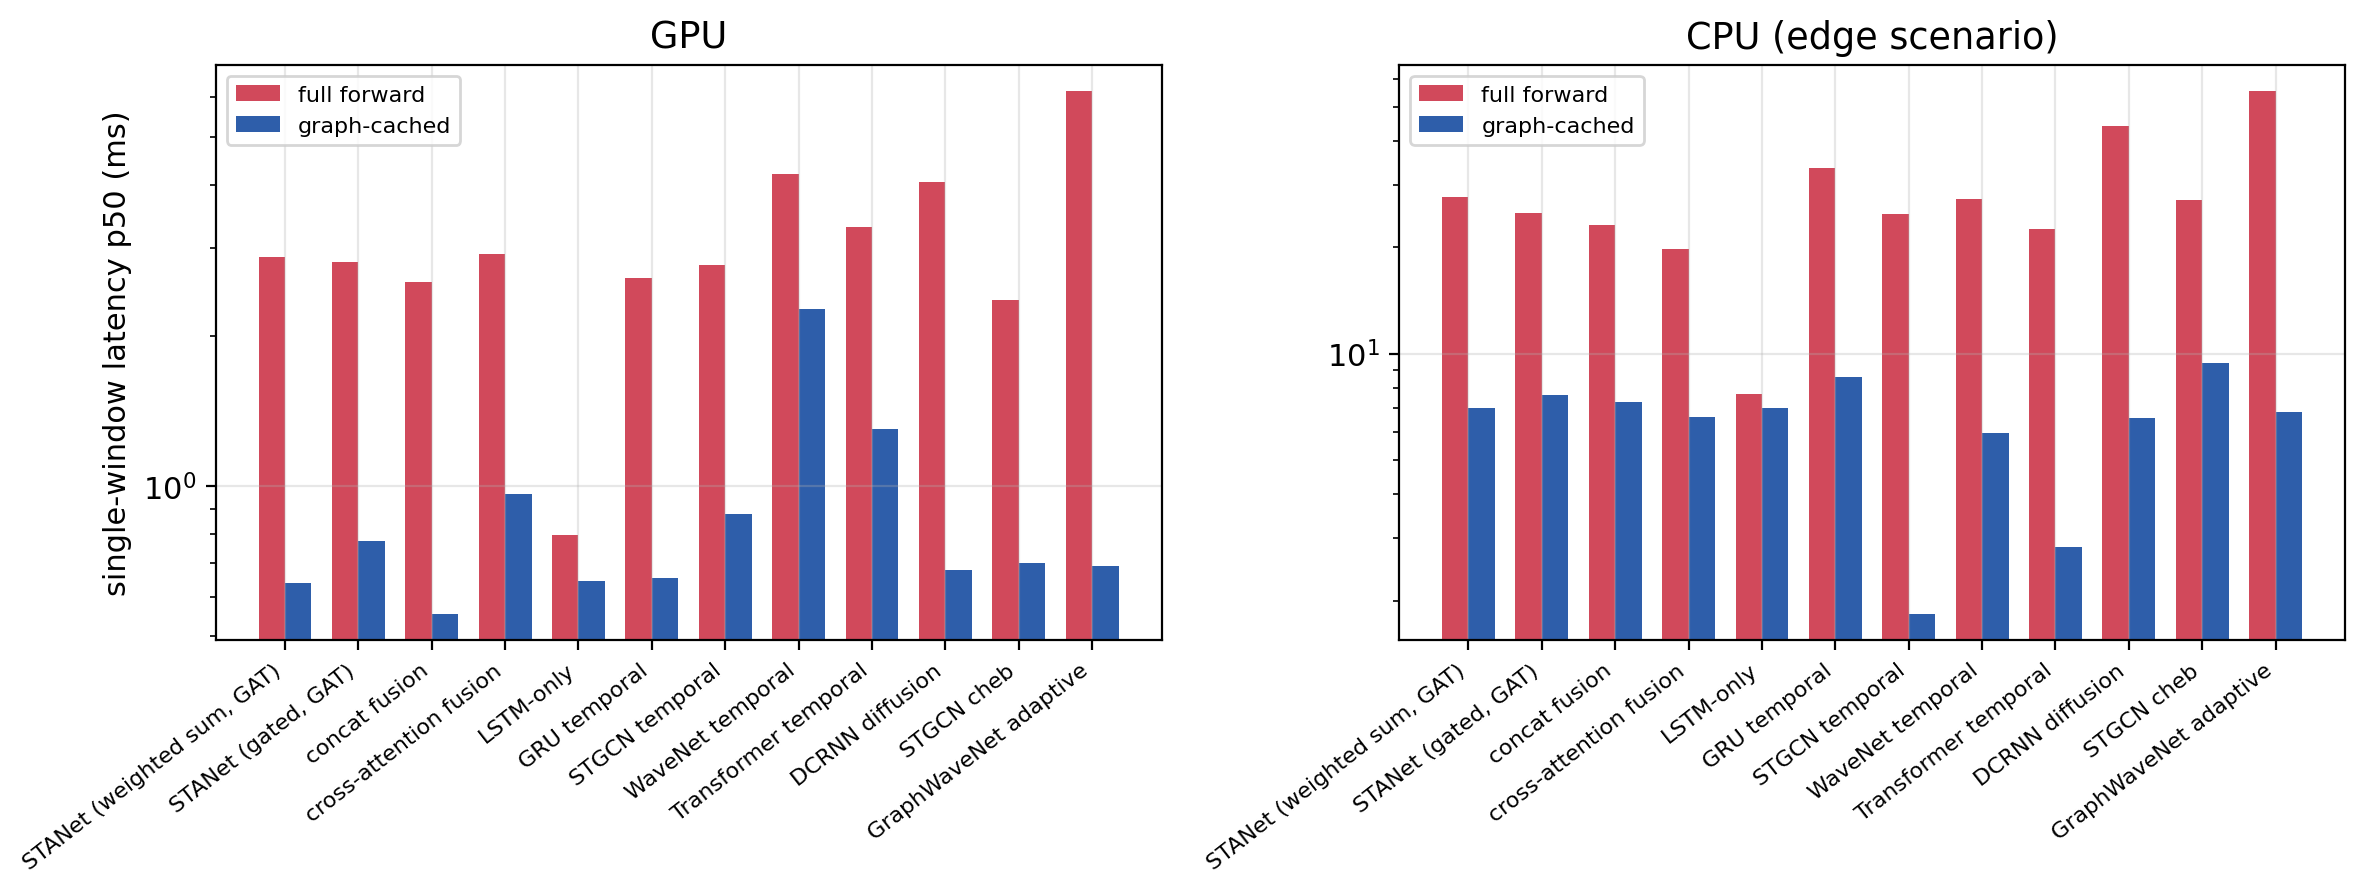
\includegraphics[width=0.98\linewidth]{fig_F6_efficiency.png}
  \caption{Single-window latency with and without graph-embedding caching, on GPU and CPU (log scale).}
  \label{fig:efficiency}
\end{figure}

The primary model contains $220{,}802$ parameters ($\approx 0.9$~MB in fp32), of which the temporal branch accounts for $200{,}704$ ($90.9\%$), the projection layers $12{,}416$, the classifier $2{,}113$, the spatial branch only $5{,}568$ ($2.5\%$), and the fusion operator a single scalar. Peak GPU memory is $66$~MB.

Despite that small share, the spatial branch dominates inference cost, because a naive implementation recomputes embeddings for all $4{,}678$ nodes on every forward pass. \textbf{Since the road network is static, node embeddings can be computed once and cached}, reducing GPU latency from $2.87$ to $0.64$~ms ($4.5\times$) and CPU latency from $27.82$ to $7.03$~ms ($4.0\times$). After caching, the hybrid model matches the temporal-only model exactly on both devices ($0.64$~ms on GPU, $7.03$~ms on CPU): once the graph forward pass is amortized, spatial context is free at inference time. This holds for every fusion operator, since all four cost at most $16{,}640$ parameters and none appears in the latency ranking.

At $27.82$~ms per uncached window on CPU ($p_{95} = 39.92$~ms), or $7.03$~ms cached ($p_{95} = 8.77$~ms), a single-core edge device could process on the order of $35$ windows per second without caching and $140$ with it, against a one-second sampling resolution. Caching is therefore not an optimization but a precondition for single-core deployment at scale. Memory is not a constraint at this model size. These figures characterize computational feasibility only; they do not address detection quality under real sensing conditions.

\subsection{Scope of the Contribution}
\label{sec:scope}
It is worth stating directly what kind of claim this paper does and does not make, because the two are easily conflated in this literature.

This is an \emph{evaluation study}. Its object is a set of design decisions---encoder pairing, fusion operator, graph construction---and its result is a statement about how much evidence a controlled comparison can actually support for each of them. It is not a report of a deployable traffic anomaly detector, and none of the numbers here should be read as an estimate of field performance. The data are simulated; the labels are, for most subtypes, threshold functions of the model's own inputs; the road network is one city; the trip count is $90$. Each of these independently rules out a deployment claim, and we make none.

What survives those limitations is the methodological finding, and it does so precisely because it is a \emph{relative} statement evaluated under a single fixed protocol: a sample-wise gate that is presented as the architectural contribution of a hybrid model does not, on this data, outperform a single learnable scalar, and the difference between the two is smaller than the variation across random seeds. That comparison does not depend on the data being real, because every variant faces the identical task, partition, budget, and decision rule. It does depend on the comparison being controlled, which is why Section~\ref{sec:protocol_note} and Section~\ref{sec:statistical_unit} are given the space they are.

Whether the same conclusion holds on field-collected trajectories is an open question that this dataset cannot answer, and we identify it in Section~\ref{sec:future_directions} as the decisive next experiment rather than implying it here.

\subsection{Threats to Validity}
\label{sec:threats}

\textbf{Synthetic data.} All findings are obtained on simulated trajectories over one city network. No real sensor data, verified incident record, or prospective stream is involved, and no claim about real-world detection performance is made.

\textbf{Label--input dependence.} Most anomaly subtypes are threshold functions of the model's own inputs (Section~\ref{sec:reference_points}). Conclusions about \emph{relative} architectural merit are unaffected, since all configurations face the same task, but absolute performance figures reflect a partly self-referential problem and should not be compared to results on independently labelled data.

\textbf{Statistical power.} This is the tightest constraint on what the paper can claim, and it is a consequence of the sampling design rather than of the analysis. Because windows overlap by $80\%$ and share a trip, the unit of analysis is the trip (Section~\ref{sec:statistical_unit}), and the dataset contains only $90$ trips: roughly $13$ of them in the fixed test partition, all $90$ across the cross-validation folds. Interval estimates on the fixed partition are therefore wide, and comparisons that appear significant at the window level frequently are not once the correct unit is used. We report both, labelled, and base conclusions on the trip-level, Holm-corrected values from the cross-validated analysis. Differences that the design cannot resolve are presented as point estimates with intervals and are not claimed as significant---including differences that would favour the architecture proposed in the earlier version of this work.

\textbf{Encoder adaptation.} STGCN, DCRNN, and Graph WaveNet are represented by their core operators rather than their full published architectures. This is necessary given the task mismatch, but the results should be read as evidence about those operators in this setting rather than as a benchmark of the published systems.

\textbf{Imputation dependence.} Roughly half of the lane counts and speed limits are author-defined defaults, which directly affects the node features available to the spatial branch. A sensitivity analysis over these defaults was not performed.

% =====================================================================
% BOLUM VIII — SONUC
% =====================================================================
\section{Conclusion and Future Work}

This study evaluated the components of a hybrid LSTM--GAT traffic anomaly detector under a controlled protocol in which one element is varied at a time and every result is reported over multiple seeds with interval estimates and paired tests.

\subsection{Summary of Findings}
\begin{itemize}
  \item \textbf{The fixed partition supports no claim at all.} It holds $4{,}799$ windows but $14$ trips. At the trip level, after Holm correction, none of sixteen comparisons is significant---including seven that are significant when windows are treated as independent. The hybrid model's own F1 on that partition carries an interval of $[0.7231, 0.9470]$.
  \item \textbf{The fusion ranking is partition-dependent, in both directions.} The sample-wise gate ranks last of four on the fixed partition and first of four under cross-validation, where no operator differs significantly from any other. We therefore make no accuracy claim for or against the gating mechanism, and we withdraw the earlier claim against it.
  \item \textbf{A reproducible collapse mode exists and is conditional.} The gate collapsed to $\mathrm{F1}=0.0715$ at one of five seeds on the fixed partition, recurring at the same seed in an independent re-run under a different backend configuration. It occurred in none of ten cross-validated runs, and it disappears on a graph construction where the spatial branch carries more standalone signal. It is a rare, conditional failure mode worth documenting for practitioners---not evidence of general inferiority.
  \item \textbf{The spatial branch shows no measurable benefit.} Under cross-validation no anomaly subtype shows a significant gain from the spatial branch after correction, and pooled F1 is highest for the control that has no spatial branch at all. A gain on abnormal-dwell detection reported in the previous version was an artifact of a pooled threshold and is withdrawn (Section~\ref{sec:subtype}); the comparison now closest to significance has the hybrid performing \emph{worse} on signal-freeze events.
  \item \textbf{Encoder choice separates along one axis only.} Graph attention exceeds Chebyshev convolution, diffusion convolution, and adaptive adjacency; the LSTM, a GRU, and a Transformer encoder finish within $0.0015$ F1 of one another. Which spatial operator is used is resolvable here; which recurrence is used is not.
  \item \textbf{Gate interpretability is seed-dependent.} The class-conditional shift in $g_{gate}$ varies in magnitude and sign across seeds and does not constitute a stable model property.
  \item \textbf{Deployment cost is removable} (Section~\ref{sec:efficiency}). Caching static node embeddings reduces single-window latency by $4.5\times$ on GPU and $4.0\times$ on CPU, after which the hybrid model matches temporal-only latency exactly.
  \item \textbf{Simple references are strong.} A zero-parameter three-threshold rule reaches $\mathrm{F1}=0.8536$ and gradient boosting on window aggregates matches the neural model to within $0.0014$ F1, with higher ROC-AUC.
\end{itemize}

\subsection{Implications}
The limitations bounding these conclusions are collected in Section~\ref{sec:threats}. The broader implication is methodological, and it has three parts that we would separate.

\textbf{The unit of analysis is not a detail.} Sliding-window evaluation is near-universal in this literature, and windows cut with a stride shorter than their length are not independent observations. Reporting window-level $p$-values under that design does not slightly overstate significance; in our case it turned sixteen non-significant comparisons into seven significant ones. Any study using overlapping windows should state its cluster structure and test at the level of the independent unit---here the trip, elsewhere the vehicle, the sensor, or the day.

\textbf{One partition cannot order architectures.} We report the same four fusion operators ranked in opposite orders on one partition and across five, with the mechanism under study finishing both last and first. Neither ordering is wrong; both are under-determined. A single grouped partition, even a well-constructed one, is a sample of size one from the space of partitions, and architectural rankings are not stable with respect to that sample.

\textbf{Error bars must be earned.} Extending our encoder benchmark from three seeds to five raised the leading configuration's standard deviation from $0.0033$ to $0.0188$ and removed two of its four significant margins. A tight standard deviation over three runs is not evidence of stability; it is a small sample of a quantity whose spread has not been measured.

We would additionally encourage reporting a rule-based or classical reference whenever labels are generated by known rules, since it bounds how much of the measured performance is attributable to learning at all---in this study, a zero-parameter rule reaches within $0.018$ F1 of every neural configuration tested.

\subsection{Future Directions}
\label{sec:future_directions}
\begin{itemize}
  \item \textbf{Dataset redesign.} Sharing road segments across trips and increasing the prevalence of context-dependent subtypes such as speed-limit violation would allow the spatial branch's contribution to be tested with adequate power---the decisive experiment that the present data cannot support.
  \item \textbf{Simulation-to-real transfer.} Findings obtained on physics-informed synthetic trajectories require domain adaptation before transfer to field data. Digital twin-assisted graph contrastive domain adaptation has shown promise for adapting simulation-derived representations to small-sample target domains \cite{gcda_bearing}; adding such a layer to the spatial branch is a natural next step for cross-city transfer.
  \item \textbf{Stabilized gating.} Since the collapse mode arises from the multiplicative form of Eq.~\ref{eq:gated_fusion}, entropy regularization on $g_{gate}$, a bounded gating range, or an auxiliary supervision signal on the gate are candidate remedies worth evaluating.
  \item \textbf{Imputation sensitivity.} Road-type-specific lane and speed-limit defaults should be varied systematically to quantify how strongly the spatial branch depends on author-defined assumptions.
  \item \textbf{Real-world and cross-city validation.} Field-collected sensor data, independently verified incidents, prospective streams, and external road networks are required before any claim of deployment suitability.
\end{itemize}

\section*{Data and Code Availability}
\label{sec:availability}
The synthetic dataset, its data card, the complete preprocessing and modelling code, the experiment scripts, every result file reported in this paper, and the script that verifies the manuscript's numbers against those files are available at \url{\repourl} and permanently archived at \texttt{doi:\zenododoi}, which resolves to the exact snapshot (\texttt{v2.0.0}) that produced every number reported here. The concept identifier \texttt{doi:\zenodoconcept} resolves to the most recent version. No real-world vehicle trajectory data was used.

The repository contains two mechanisms that support the internal consistency of the tables reported here. First, every result file carries a \emph{protocol stamp}: a hash over the seed set, epoch budget, patience, batch size, learning rate, scheduler, dropout, checkpoint criterion, threshold rule, cuDNN flags, window length, stride, split seed, and library versions. Scripts that consume another script's results assert that the stamps match and abort otherwise. Second, configurations that appear in more than one table are trained once and cached under their protocol stamp, so those tables read the same run rather than two independently trained runs that are assumed to agree. Section~\ref{sec:protocol_note} describes why these mechanisms were introduced.

Because several anomaly subtypes are defined as threshold functions of the model's input channels, a zero-parameter rule-based classifier is reported alongside all learned models as a reference point.

% Kaynakca elle yazilmis bir thebibliography ortami olarak tutuluyor
% (orijinal PDF'ten cikarilip atif anahtarlariyla eslestirildi; bkz. _build_refs.py).
% BibTeX kullanilmiyor: stanet.bib mevcut degil.
\begin{thebibliography}{99}
\itemsep=0pt
\bibitem{huang_multivariate_2024} X. Huang, N. Chen, Z. Deng, and S. Huang, “Multivariate time series anomaly detection via dynamic graph attention network and Informer,” Applied Intelligence, vol. 54, no. 17-18, pp. 7636–7658, Sep. 2024. [Online]. Available: https://link.springer.com/10.1007/ s10489-024-05575-y
\bibitem{sun_framework_2025} M. Duan, S. Sun, and M. Liu, “A multimodal deep fusion framework for highway traffic anomaly detection,” Scientific Reports, vol. 15, p. 33573, Sep. 2025. [Online]. Available: https://www.nature.com/articles/ s41598-025-18671-x
\bibitem{nguyen_spatiotemporal_2026} H. D. Nguyen, A. T.-H. Nguyen, and T.-H. Do, “Spatiotemporal traffic prediction in Dublin: Volume, speed, and influencing factors,” Engineering Applications of Artificial Intelligence, vol. 166, p. 113602, Feb. 2026. [Online]. Available: https://linkinghub.elsevier.com/retrieve/ pii/S0952197625036346
\bibitem{liang_anomaly_2025} Q. Liang, L. Cong, and H. Du, “Anomaly traffic detection in heterogeneous lightweight networks based on spatio-temporal features,” The Journal of Supercomputing, vol. 81, no. 5, p. 690, Apr. 2025. [Online]. Available: https://link.springer.com/10.1007/s11227-025-07189-8
\bibitem{cui_lane-flow-learning_2026} H. Cui, K. Xiao, H. Wang, and X. Zhang, “Lane-flow-learning based autonomous vehicle trajectory prediction using spatial–temporal fusion attention,” Information Sciences, vol. 737, p. 123134, May 2026. [Online]. Available: https://linkinghub.elsevier.com/retrieve/pii/ S0020025526000654
\bibitem{gcda_bearing} C. Dai, D. He, Z. Jin, X. Zhang, G. Chen, J. Wu, J. Zhao, and Y. Xu, “Digital twin-assisted graph contrastive domain adaptation for small-sample bearing fault diagnosis,” Structural Health Monitoring, Apr. 2026, art. no. 14759217261440798. [Online]. Available: https://doi.org/10.1177/14759217261440798
\bibitem{zhang_automatic_2022} H. Zhang, S. Zhao, R. Liu, W. Wang, Y. Hong, and R. Hu, “Automatic Traffic Anomaly Detection on the Road Network with Spatial-Temporal Graph Neural Network Representation Learning,” Wireless Communications and Mobile Computing, vol. 2022, no. 1, p. 4222827, Jan. 2022. [Online]. Available: https://onlinelibrary.wiley.com/ doi/10.1155/2022/4222827 15
\bibitem{zhang_traffic_2025} Y. Zhang, S. Yang, H. Wang, Y. Cheng, J. Wang, L. Cao, and Z. An, “A traffic flow forecasting method based on hybrid spatial–temporal gated convolution,” International Journal of Machine Learning and Cybernetics, vol. 16, no. 3, pp. 1805–1817, Mar. 2025. [Online]. Available: https://link.springer.com/10.1007/s13042-024-02364-4
\bibitem{ren_graph_2024} Z. Ren, X. Li, J. Peng, K. Chen, Q. Tan, X. Wu, and C. Shi, “Graph autoencoder with mirror temporal convolutional networks for traffic anomaly detection,” Scientific Reports, vol. 14, no. 1, p. 1247, Jan. 2024. [Online]. Available: https://www.nature.com/articles/s41598-024-51374-3
\bibitem{li_graph_2023} H. Li, Y. Ma, X. Wang, and Z. Li, “Graph Spatiotemporal Pattern Learning Network for Real-Time Road Network Traffic Abnormal Incident Detection,” Transportation Research Record: Journal of the Transportation Research Board, vol. 2677, no. 12, pp. 815–829, Dec. 2023. [Online]. Available: https://journals.sagepub.com/doi/10.1177/ 03611981231170004
\bibitem{park_graph_2025} D. Park, S.-S. Choi, D. Lim, and Y.-S. Kang, “Graph Multi- Resolution Transformer for Road Traffic Anomaly Detection,” IEEE Access, vol. 13, pp. 27 428–27 437, 2025. [Online]. Available: https://ieeexplore.ieee.org/document/10872917/
\bibitem{chen_enhancing_2026} J. Chen, H. Chen, and H. Lu, “Enhancing Road Safety and Sustainability: A Multi-Scale Temporal Model for Vehicle Trajectory Anomaly Detection in Road Network Interactions,” Sustainability, vol. 18, no. 2, p. 597, Jan. 2026. [Online]. Available: https://www.mdpi.com/2071-1050/18/2/597
\bibitem{zhong_multi-factor_2025} R. Zhong, B. Hu, F. Wang, Y. Feng, Z. Li, X. Song, Y. Wang, S. Lou, and J. Tan, “Multi-factor embedding GNN-based traffic flow prediction considering intersection similarity,” Neurocomputing, vol. 620, p. 129193, Mar. 2025. [Online]. Available: https://linkinghub.elsevier. com/retrieve/pii/S0925231224019647
\bibitem{pan_dc-stgcn_2021} C. Pan, J. Zhu, Z. Kong, H. Shi, and W. Yang, “DC-STGCN: Dual-Channel Based Graph Convolutional Networks for Network Traffic Forecasting,” Electronics, vol. 10, no. 9, p. 1014, Apr. 2021. [Online]. Available: https://www.mdpi.com/2079-9292/10/9/1014
\bibitem{chang_stfdsgcn_2025} J. Chang, J. Yin, Y. Hao, and C. Gao, “STFDSGCN: Spatio- Temporal Fusion Graph Neural Network Based on Dynamic Sparse Graph Convolution GRU for Traffic Flow Forecast,” Sensors, vol. 25, no. 11, p. 3446, May 2025. [Online]. Available: https: //www.mdpi.com/1424-8220/25/11/3446
\bibitem{zhou_hybrid_2022} L. Zhou, Q. Zeng, and B. Li, “Hybrid Anomaly Detection via Multihead Dynamic Graph Attention Networks for Multivariate Time Series,” IEEE Access, vol. 10, pp. 40 967–40 978, 2022. [Online]. Available: https://ieeexplore.ieee.org/document/9758699/
\bibitem{taheri_sarteshnizi_applicability_2026} I. Taheri Sarteshnizi, M. Sarvi, S. Asadi Bagloee, and N. Nassir, “On the applicability of time series anomaly detection methods to real-world traffic volume data,” Transportation Research Part C: Emerging Technologies, vol. 184, p. 105536, Mar. 2026. [Online]. Available: https://linkinghub.elsevier.com/retrieve/pii/S0968090X26000240
\bibitem{hu_dynamic_2026} C. Hu, Y. Wang, X. Zhang, M. Zheng, G. Feng, J. Liu, and Y. Kang, “Dynamic Graph Neural Network-Transformer-LSTM Based Multi-Scale Spatio-Temporal Traffic Forecasting,” International Journal of Intelligent Transportation Systems Research, Feb. 2026. [Online]. Available: https://link.springer.com/10.1007/s13177-025-00623-4
\bibitem{zhu_spatio-temporal_2026} L. Zhu, Q. Zhang, X. Jian, Y. Yang, and L. Li, “Spatio-temporal traffic accidents detection via graph based generative adversarial network,” Engineering Applications of Artificial Intelligence, vol. 165, p. 113488, Feb. 2026. [Online]. Available: https://linkinghub.elsevier.com/retrieve/ pii/S0952197625035195
\bibitem{xia_attention-based_2023} D. Xia, B. Shen, J. Geng, Y. Hu, Y. Li, and H. Li, “Attention- based spatial–temporal adaptive dual-graph convolutional network for traffic flow forecasting,” Neural Computing and Applications, vol. 35, no. 23, pp. 17 217–17 231, Aug. 2023. [Online]. Available: https://link.springer.com/10.1007/s00521-023-08582-1
\bibitem{wang_multi-scale_2025} J. Wang, K. Liu, H. Li, Q. Gao, X. Wang, and Y. Gong, “Multi- Scale Temporal Features-Based Hybrid LSTM-GAT for Traffic Flow Prediction,” IEEE Internet of Things Journal, pp. 1–1, 2025. [Online]. Available: https://ieeexplore.ieee.org/document/11127181/
\bibitem{feng_traffic_2024} J. Feng, Y. Zhang, X. Piao, Y. Hu, and B. Yin, “Traffic Anomaly Detection based on Spatio-Temporal Hypergraph Convolution Neural Networks,” Physica A: Statistical Mechanics and its Applications, vol. 646, p. 129891, Jul. 2024. [Online]. Available: https://linkinghub.elsevier. com/retrieve/pii/S037843712400400X
\bibitem{ma_utfp-ad_2025} Y. Ma, Y. Nie, J. Guo, J. Zhu, F. Li, Q. Xie, and A. V. Vasilakos, “UTFP-AD: Urban Traffic Flow Pattern Anomaly Detection Using Spatiotemporal Data,” IEEE Transactions on Intelligent Transportation Systems, vol. 26, no. 10, pp. 15 970–15 984, Oct. 2025. [Online]. Available: https://ieeexplore.ieee.org/document/11029517/
\bibitem{guo_crfpi-net_2026} W. Guo, W. Xu, C. Yang, Z. Zhao, X. Gao, W. Yao, and S. Jin, “CRFPI-Net: context-aware risk feature perception and inference network for pixel-level urban traffic risk mapping,” Advanced Engineering Informatics, vol. 71, p. 104299, Apr. 2026. [Online]. Available: https://linkinghub.elsevier.com/retrieve/pii/S1474034625011929
\bibitem{he_c_2025} Q. He, F. Zhang, G. Bian, W. Zhang, and Z. Li, “C-lstm traffic anomaly detection model based on attention mechanism,” Concurrency and Computation: Practice and Experience, vol. 37, no. 25-26, p. e70314, Nov. 2025. [Online]. Available: https: //onlinelibrary.wiley.com/doi/10.1002/cpe.70314
\bibitem{hirata_traffic_2025} K. Hirata, Y. Kawasaki, and T. Yoshida, “A Traffic Anomaly Detection Method Using Traffic Flow Vectors During Heavy Rainfall,” International Journal of Intelligent Transportation Systems Research, vol. 23, no. 1, pp. 91–103, Apr. 2025. [Online]. Available: https://link.springer.com/10.1007/s13177-024-00438-9
\bibitem{chen_gms_2026} X. Chen, G. Gu, and X. Ning, “GMS: Graph-Guided Multi-Modal Spatio- Temporal Fusion model for trajectory prediction in autonomous driving,” Neurocomputing, vol. 661, p. 132010, Jan. 2026. [Online]. Available: https://linkinghub.elsevier.com/retrieve/pii/S0925231225026827
\bibitem{wen_hdsvt_2025} D. Wen et al., “HDSVT: High-Density Semantic Vehicle Trajectory Dataset Based on a Cosmopolitan City Bridge,” Scientific Data, vol. 13, no. 1, p. 5, Dec. 2025.
\bibitem{feng_traffic_2024_dup2} J. Feng, Y. Zhang, X. Piao, Y. Hu, and B. Yin, “Traffic Anomaly Detection based on Spatio-Temporal Hypergraph Convolution Neural Networks,” Physica A, vol. 646, p. 129891, Jul. 2024.
\bibitem{yu_spatio-temporal_2018} B. Yu, H. Yin, and Z. Zhu, “Spatio-temporal graph convolutional networks: A deep learning framework for traffic forecasting,” in Proc. IJCAI, 2018, pp. 3634–3640.
\bibitem{li_diffusion_2018} Y. Li, R. Yu, C. Shahabi, and Y. Liu, “Diffusion convolutional recurrent neural network: Data-driven traffic forecasting,” in Proc. ICLR, 2018.
\bibitem{wu_graph_2019} Z. Wu, S. Pan, G. Long, J. Jiang, X. Chang, and C. Zhang, “Graph wavenet for deep spatial-temporal graph modeling,” in Proc. IJCAI, 2019, pp. 1907–1913.
\bibitem{francies_framework_2025} M. L. Francies, A. T. Khalil, H. M. Amer, and M. M. Ata, “A framework for continual learning in real-time traffic forecasting utilizing spatial–temporal graph convolutional recurrent networks,” Complex \& Intelligent Systems, vol. 11, no. 10, p. 420, Oct. 2025.
\bibitem{pipes_car_following_1967} L. A. Pipes, “Car following models and the fundamental diagram of road traffic,” Transportation Research, vol. 1, no. 1, pp. 21–29, 1967.
\bibitem{aashto_green_book_2018} AASHTO, A Policy on Geometric Design of Highways and Streets, 2018.
\end{thebibliography}

\end{document}
